%=====================================================================
%  MS in Data Science & Agentic AI — Team Project Report Template
%  Northwestern University (School of Professional Studies style)
%
%  NOTE: This is a faculty-prepared template that follows Northwestern's
%  visual identity (Northwestern Purple, Pantone 2685C / RGB 78,42,132).
%  It is not an official University document; check current SPS
%  submission rules before use. Fonts fall back to Times/Helvetica so it
%  compiles on any TeX Live with pdflatex.
%
%  Build:  pdflatex main -> bibtex main -> pdflatex main -> pdflatex main
%          (or simply:  latexmk -pdf nu_ms_project_template.tex)
%=====================================================================
\documentclass[11pt,letterpaper,oneside]{report}

%---------------------------------------------------------------------
% Packages
%---------------------------------------------------------------------
\usepackage[utf8]{inputenc}
\usepackage[T1]{fontenc}
\usepackage{mathptmx}                       % Times-like body font
\usepackage[scaled=0.92]{helvet}            % Helvetica-like sans for headings
\usepackage[margin=1in]{geometry}
\usepackage{setspace}
\usepackage{xcolor}
\usepackage{graphicx}
\usepackage{amsmath,amssymb}
\usepackage{booktabs}
\usepackage{tabularx}
\usepackage{longtable}
\usepackage{caption}
\usepackage{subcaption}
\usepackage{enumitem}
\usepackage{titlesec}
\usepackage{fancyhdr}
\usepackage{listings}
\usepackage{algorithm}
\usepackage{algpseudocode}
\usepackage[numbers,sort&compress]{natbib}
\usepackage{url}
\usepackage[hidelinks]{hyperref}
\usepackage{lipsum}                          % dummy text — remove in final
\usepackage{tikz}
\usepackage{placeins}                        % \FloatBarrier keeps figures in their section
\usetikzlibrary{positioning,arrows.meta,fit,backgrounds}
\usepackage[T1]{fontenc}
\usepackage{xcolor}
\usetikzlibrary{arrows.meta,calc,positioning}

%---------------------------------------------------------------------
% Northwestern colours
%---------------------------------------------------------------------
\definecolor{NUPurple}{RGB}{78,42,132}
\definecolor{NUPurple60}{RGB}{164,149,195}
\definecolor{NUGrey}{RGB}{113,108,110}
\definecolor{CodeBG}{RGB}{245,243,249}

%---------------------------------------------------------------------
% Project metadata — EDIT THESE
%---------------------------------------------------------------------
\newcommand{\ProjectTitle}{LensRAG - Long-range ENriched Search for RAG}
\newcommand{\ProjectSubTitle}{Corpus-Level Aggregation Queries over Enterprise Documents}
\newcommand{\Programme}{MTech in Data Science}
\newcommand{\Course}{Capstone Project}
\newcommand{\Term}{Batch A, January 2025}
\newcommand{\Advisor}{Dr.\ Narayana Darapaneni \& Anwesh Reddy Paduri}
\newcommand{\TeamName}{mTechPesJan2025AGrp5}
\newcommand{\SubmissionDate}{December 2026}
\newcommand{\RepoURL}{https://github.com/brags-labs/corpusrag}
\newcommand{\ProjectNumber}{Project 1}

%---------------------------------------------------------------------
% Heading styles
%---------------------------------------------------------------------
\titleformat{\chapter}[display]
  {\sffamily\bfseries\color{NUPurple}}
  {\filleft\fontsize{60}{60}\selectfont\color{NUPurple60}\thechapter}
  {-8pt}{\filleft\Huge}
\titlespacing*{\chapter}{0pt}{-20pt}{30pt}
\titleformat{\section}{\sffamily\Large\bfseries\color{NUPurple}}{\thesection}{1em}{}
\titleformat{\subsection}{\sffamily\large\bfseries\color{NUPurple}}{\thesubsection}{1em}{}
\titleformat{\subsubsection}{\sffamily\normalsize\bfseries\color{NUGrey}}{\thesubsubsection}{1em}{}

%---------------------------------------------------------------------
% Header / footer
%---------------------------------------------------------------------
\pagestyle{fancy}
\fancyhf{}
\renewcommand{\headrulewidth}{0.4pt}
\renewcommand{\headrule}{\hbox to\headwidth{\color{NUPurple}\leaders\hrule height \headrulewidth\hfill}}
\fancyhead[L]{\small\sffamily\color{NUGrey}\Programme}
\fancyhead[R]{\small\sffamily\color{NUGrey}\ProjectNumber}
\fancyfoot[C]{\small\sffamily\thepage}
\fancypagestyle{plain}{\fancyhf{}\fancyfoot[C]{\small\sffamily\thepage}\renewcommand{\headrulewidth}{0pt}}

%---------------------------------------------------------------------
% Captions, lists, code
%---------------------------------------------------------------------
\captionsetup{font=small,labelfont={bf,color=NUPurple},labelsep=period}
\setlist{nosep,leftmargin=*}
\lstset{
  basicstyle=\ttfamily\small, backgroundcolor=\color{CodeBG},
  frame=single, rulecolor=\color{NUPurple60}, breaklines=true,
  keywordstyle=\color{NUPurple}\bfseries, commentstyle=\color{NUGrey}\itshape,
  showstringspaces=false, numbers=left, numberstyle=\tiny\color{NUGrey}
}
\onehalfspacing
\setlength{\parskip}{4pt}

%=====================================================================
\begin{document}

%---------------------------------------------------------------------
% TITLE PAGE
%---------------------------------------------------------------------
\begin{titlepage}
  \thispagestyle{empty}
  \noindent{\color{NUPurple}\rule{\textwidth}{6pt}}
  \vspace{6pt}

  \noindent{\sffamily\large\color{NUGrey} PES UNIVERSITY\\
  School of Data Sciences \\
  \Programme}


  \vspace{0.4cm}
  \noindent{\sffamily\bfseries\LARGE\color{NUPurple}\ProjectTitle}
  
  \noindent{\sffamily\bfseries\large\color{NUGrey}\ProjectSubTitle}

  \vspace{1cm}
  \noindent{\large Team Project Report}\\[4pt]
  \noindent{\Course\ \textbar\ \Term}

  \vspace{1.8cm}
  \noindent{\sffamily\bfseries\color{NUPurple}\TeamName}

  \vspace{0.3cm}
  \noindent
  \begin{tabularx}{\textwidth}{@{}l X l@{}}
    \toprule
    \textbf{Team member} & \textbf{Role} & \textbf{Roll No.} \\
    \midrule
    Alok Kumar  & Research design         & PES2PGE25DS005 \\
    Bhibu Prasanna Mohapatra  & Research design                & PES2PGE25DS014  \\
    Gautam Pandey &      Research design                & PES2PGE25DS022 \\
    Raghavendra Rajarao  & Research design     & PES2PGE25DS069 \\
    Shivakumar Athreya  & Research design & PESPGE2025DS084 \\
    \bottomrule
  \end{tabularx}

  \vspace{1.2cm}
  \noindent\textbf{Faculty Advisor:} \Advisor

  \noindent\textbf{Code \& data repository:} \url{\RepoURL}

  \vfill
  \noindent{\sffamily\color{NUGrey}\SubmissionDate}
  \hfill
  {\sffamily\color{NUGrey} Bangalore }

  \noindent{\color{NUPurple}\rule{\textwidth}{2pt}}
\end{titlepage}

%---------------------------------------------------------------------
% FRONT MATTER
%---------------------------------------------------------------------
\pagenumbering{roman}

\chapter*{Abstract}
\addcontentsline{toc}{chapter}{Abstract}
Write 250--300 words. State the problem and why it matters to industry
(cite the market driver), the gap in prior work, what you built or measured,
the headline quantitative result (e.g., ``the gateway reduced tool-poisoning
success from 61\% to 4\% at a 7\% task-completion cost''), and the released
artifact (benchmark, dataset, reference architecture).

\vspace{1em}
\noindent\textbf{Keywords:} agentic AI; Model Context Protocol; retrieval-augmented generation; evaluation; LLMOps.

\chapter*{Declaration and AI-Use Disclosure}
\addcontentsline{toc}{chapter}{Declaration and AI-Use Disclosure}
We declare that this report is our own work, that all sources are cited, and
that all experiments reported were actually executed as described.

\medskip
\noindent\textbf{Generative-AI tools used.} List every tool (e.g., Claude, ChatGPT,
Copilot) and for what purpose (`literature search, code drafting, proofreading,
figure generation). State which parts of the text or code were AI-drafted and
how they were verified. Per programme policy, AI tools may not be used to
fabricate data, results or references.

\medskip
\noindent\textbf{Data and ethics.} No PII information is used., These are HR policy related mock data.

\chapter*{Acknowledgements}
\addcontentsline{toc}{chapter}{Acknowledgements}
Optional.

\tableofcontents
\listoffigures
\listoftables

\chapter*{Abbreviations}
\addcontentsline{toc}{chapter}{Abbreviations}
\begin{tabularx}{\textwidth}{@{}lX@{}}
A2A & Agent2Agent protocol \\
ADLC & Agent development life cycle \\
HITL & Human-in-the-loop \\
LLMOps / AgenticOps & Operations practices for LLM- and agent-based systems \\
MCP & Model Context Protocol \\
RAG / CRAG & Retrieval-augmented generation / corrective RAG \\
\end{tabularx}

\clearpage
\pagenumbering{arabic}

%---------------------------------------------------------------------
% MAIN BODY
%---------------------------------------------------------------------
%=====================================================================
%  Chapter 1 — Introduction
%  Drop-in replacement for the "Introduction" chapter in
%  project_template.tex. Uses references.bib (natbib, plainnat).
%  Items marked TODO need the team's own figures or decisions.
%=====================================================================
\chapter{Introduction}
\label{ch:intro}

\section{Context and Motivation}
\label{sec:context}
The objective of this research is to develop a novel architecture and
algorithm for Retrieval-Augmented Generation (RAG) that reliably and
accurately answers corpus-level queries, such as counting, summarising themes
or tracking sentiment shifts, without converting the documents into
structured SQL tables.

Standard RAG systems are good at answering specific queries, where the answer
can be found in one or a few documents. However, they perform poorly on
questions that require collating information by scanning all the documents in
the corpus, for example ``How many documents mention a data breach?'' or
``What are the main themes across all reviews?''. \citet{luo2025globalrag}
demonstrate that existing RAG architectures perform poorly on such global
queries, producing fluent and confident but factually wrong outputs. This
failure is especially critical in high-stakes domains such as healthcare, law
and finance, where global reasoning over entire document collections carries
significant decision-making value.

Ongoing research in this field has shown improvements on aggregation queries.
Structured RAG (S-RAG) converts the documents into database records while
they are being indexed, so that a question can later be answered by an SQL
query \citep{koshorek2025srag}. SParC-RAG (Adaptive Sequential--Parallel
Scaling with Context Management) takes a different route, mixing step-by-step
refinement with several sub-queries explored in parallel, all sharing one
managed context \citep{yang2026sparcrag}. These results highlight an opportunity for further
research. The present work aims to identify improvements during embedding and
vector-based retrieval by including contextual information that supports
long-range contextualisation, with the potential to overcome current RAG
limitations on aggregation queries.

The research is grounded in the enterprise human-resources (HR) domain.
Employees and HR staff routinely ask cross-cutting questions about
entitlements across countries, employee categories and policy versions, and
policy corpora contain features that make such questions difficult:
country-specific addenda, exceptions attached to general rules,
cross-references between chapters, and superseded versions of the same policy
that remain in circulation. We therefore construct an HR policy corpus for a
fictional multinational, BragsLabs. Its
core is a 47-chapter policy manual (about 41{,}000 words and 130 tables)
covering global policies, cross-border rules and addenda for ten countries,
extended with earlier policy versions, circulars, and synthetic helpdesk
tickets, grievances and exit notes. A local question on this corpus, such as
``How many days of paternity leave do employees in India receive?'', is
answered by a single section of the India addendum. A global question, such
as ``How many countries offer more than 20 days of annual leave?'' or ``Which
three countries have the longest notice period?'', requires finding the
relevant clause in every country addendum, extracting comparable values and
computing an exact count or ranking. Thematic and sentiment questions, such
as ``What are the most common themes in grievances raised this year?'' or
``How has sentiment in exit notes changed since the revised leave policy?'',
require reading across hundreds of free-text records. The research proceeds in
three stages:
\begin{enumerate}
  \item \textbf{Baseline.} Build a domain-specific test set of local and
  aggregation queries over the BragsLabs corpus, with ground-truth answers
  derived independently of the systems under test, and run standard top-$k$
  RAG and long-context prompting on it. This documents where and how the
  baselines fail and provides the comparative reference for later stages.
  \item \textbf{Architecture and algorithm.} Design a retrieval and
  aggregation method (Section~\ref{sec:approach}) that enriches each chunk
  with its document context before embedding, retrieves for coverage rather
  than only relevance, and computes aggregate answers deterministically at
  query time, without building a SQL schema over the corpus.
  \item \textbf{Evaluation.} Compare the proposed method with the baselines,
  and with published approaches such as GlobalRAG \citep{luo2025globalrag}
  where feasible, on the same test set and on progressively larger versions
  of the corpus.
\end{enumerate}

The performance evaluation will show whether the proposed method improves
answers to corpus-level queries over standard RAG baselines. The evaluation
framework will include an aggregation accuracy metric (correctness of the
aggregated answer), a hit rate or retrieval recall metric (the share of
required evidence that was retrieved), and a faithfulness rate (the share of
statements in the generated response that are supported by facts in the
corpus). It will also report token cost per query and latency, giving a
comprehensive performance report on the sample datasets.

\subsection{Recommended Approach}
\label{sec:approach}

We propose \emph{LensRAG} (Long-range ENriched Search for
Retrieval-Augmented Generation). The method keeps the corpus as text and a vector
index, as in standard RAG, and changes three things: what is embedded, how
much is retrieved, and where the final computation happens. Unlike S-RAG
\citep{koshorek2025srag}, it does not define a schema or load the corpus into
a database at ingestion. The only structured data are short-lived evidence
records created for a single query, each pointing to the passage it came
from.

\paragraph{Ingestion: context-enriched indexing.}
Each document is parsed into a tree of chapters, sections and tables, so that
tables are not split across chunks. Before a chunk is embedded, a short
contextual header is prepended to it: the document title, the section path
(for example \emph{HR Manual $\rangle$ Ch.~40 India Addendum $\rangle$ 40.3
Leave}), the scope (country, employee category), the version and effective
date, and the entities it mentions. This gives each chunk long-range context
that is otherwise lost when a document is split, so that a clause such as
``this applies for 10 days'' can be matched to the right country and policy.
Chunks are indexed in a hybrid index (BM25 and dense embeddings), and their
metadata in an entity list that records, for example, every country that has
an addendum.

\paragraph{Query time.}
Figure~\ref{fig:pipeline} summarises the query pipeline. A router classifies
the query. Local queries follow the standard retrieve--rerank--generate path.
For global queries, the query is expanded into one sub-query per relevant
entity, taken from the entity list, and retrieval continues until no new
relevant entities are found, rather than stopping at a fixed $k$. An LLM then
checks each candidate passage against the query condition and extracts the
required value with its supporting evidence span. Counts, extrema, rankings
and top-$k$ lists are computed in code over these records. Theme and
sentiment queries instead use a map--reduce step: each passage is labelled
with themes or sentiment, labels are grouped (for sentiment shift, by time
period), and the groups are summarised. Finally, a verification step checks
completeness against the entity list, flags conflicting values from different
sections or policy versions, and confirms that every statement in the answer
is backed by an evidence span.
The method is model-agnostic: each stage in Figure~\ref{fig:pipeline} names
the role of the model it needs, and candidate open-source and API models for
each role are listed in Table~\ref{tab:models} (Section~\ref{sec:architecture}).


\begin{figure}[p]
\centering
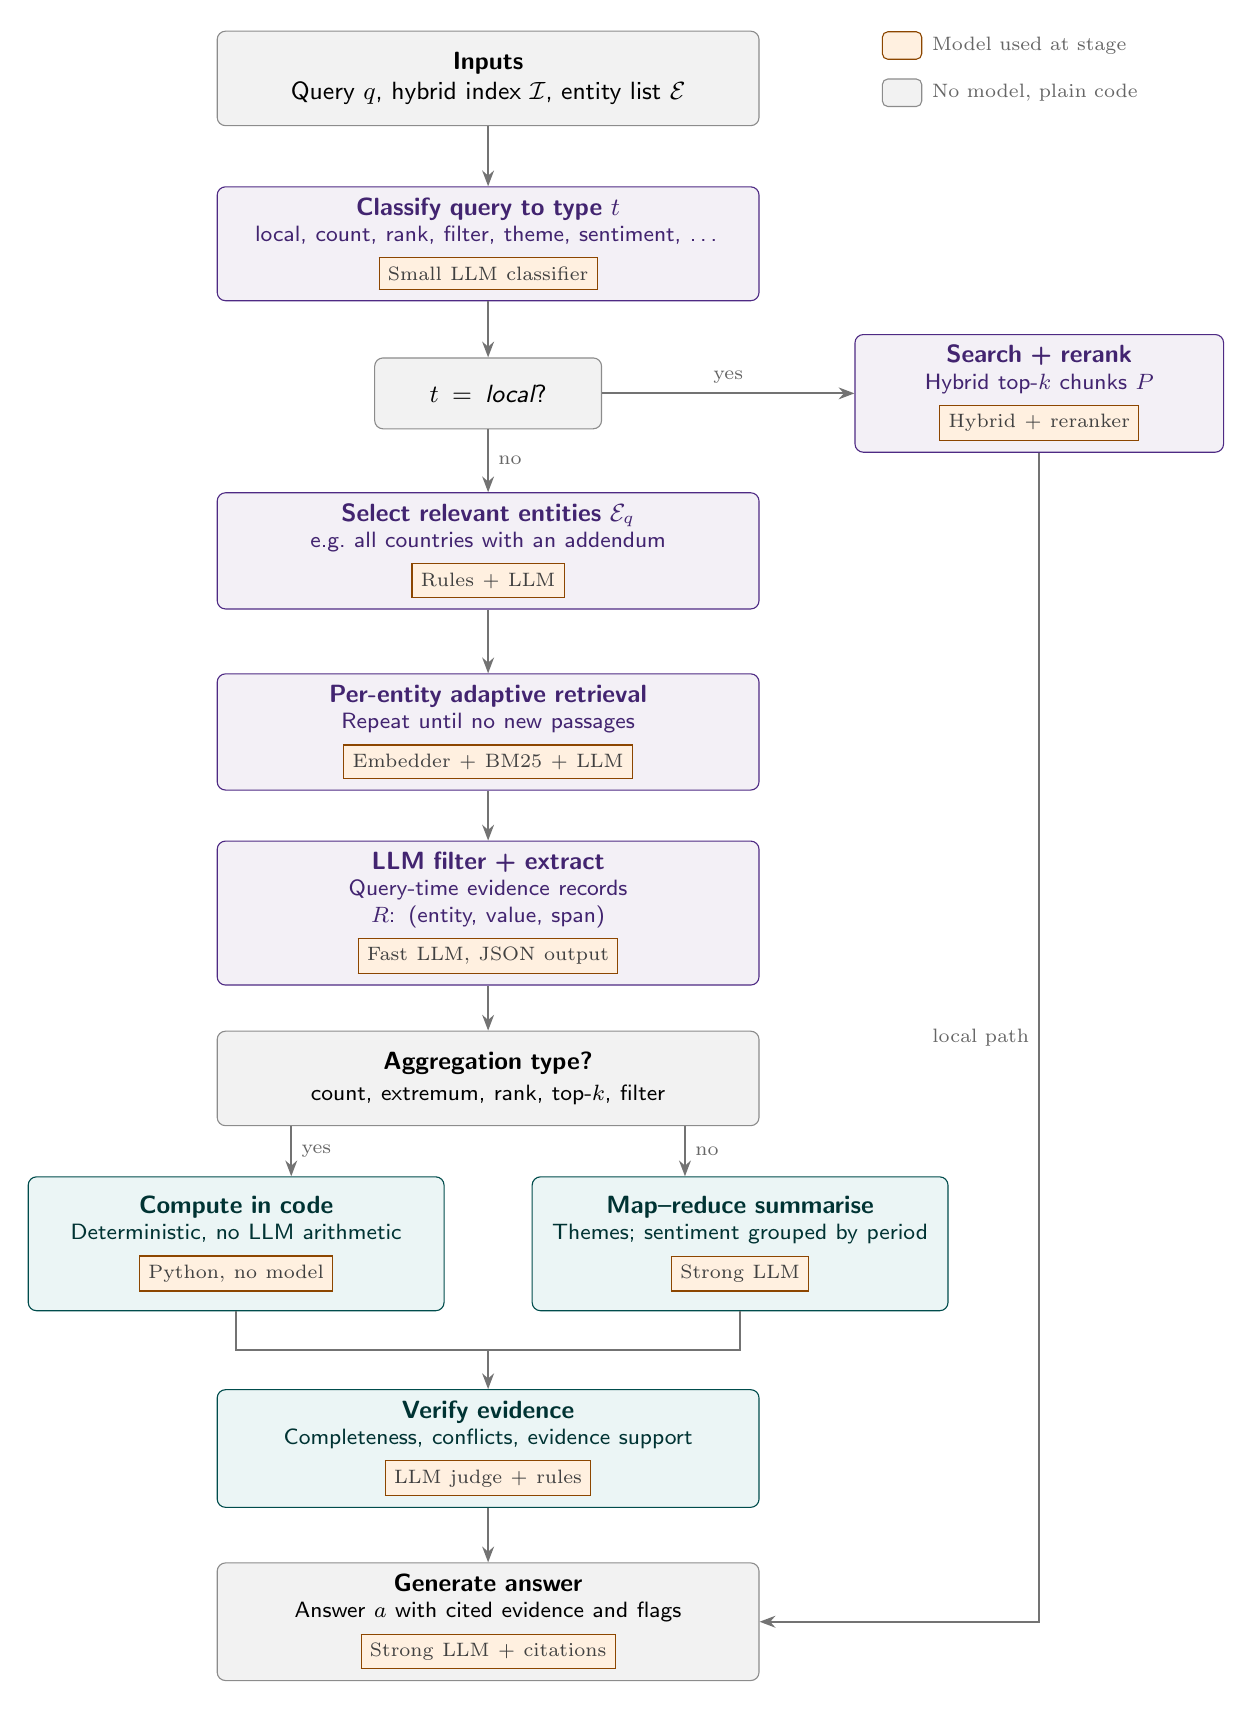
\begin{tikzpicture}[
  font=\small\sffamily,
  every node/.style={align=center},
  base/.style={rounded corners=3pt, minimum height=12mm, inner sep=4pt, text width=66mm},
  stage/.style={base, draw=NUPurple, fill=NUPurple!7, text=NUPurple!85!black},
  plain/.style={base, draw=black!45, fill=black!5},
  check/.style={base, draw=teal!60!black, fill=teal!8, text=teal!40!black},
  arr/.style={-{Stealth[length=2mm]}, draw=black!55, thick},
  lbl/.style={font=\scriptsize\rmfamily, text=black!60}
]
  % tag for the model used at each stage
  \newcommand{\mtag}[1]{\\[3pt]\fcolorbox{orange!55!black}{orange!12}{\scriptsize\rmfamily\color{black!75}#1}}
  \newcommand{\ttl}[1]{\textbf{#1}\\}

  \node[plain] (in) at (0,0) {\ttl{Inputs}Query $q$, hybrid index $\mathcal{I}$, entity list $\mathcal{E}$};
  \node[stage] (cls) at (0,-2.1) {\ttl{Classify query to type $t$}\footnotesize local, count, rank, filter, theme, sentiment, \ldots\mtag{Small LLM classifier}};
  \node[plain, text width=26mm, minimum height=9mm] (dec) at (0,-4.0) {$t=\textit{local}$?};
  \node[stage, text width=44mm] (loc) at (7.0,-4.0) {\ttl{Search + rerank}\footnotesize Hybrid top-$k$ chunks $P$\mtag{Hybrid + reranker}};
  \node[stage] (ent) at (0,-6.0) {\ttl{Select relevant entities $\mathcal{E}_q$}\footnotesize e.g.\ all countries with an addendum\mtag{Rules + LLM}};
  \node[stage] (ret) at (0,-8.3) {\ttl{Per-entity adaptive retrieval}\footnotesize Repeat until no new passages\mtag{Embedder + BM25 + LLM}};
  \node[stage] (ext) at (0,-10.6) {\ttl{LLM filter + extract}\footnotesize Query-time evidence records $R$: (entity, value, span)\mtag{Fast LLM, JSON output}};
  \node[plain] (agt) at (0,-12.7) {\ttl{Aggregation type?}\footnotesize count, extremum, rank, top-$k$, filter};
  \node[check, text width=50mm, minimum height=17mm] (cmp) at (-3.2,-14.8) {\ttl{Compute in code}\footnotesize Deterministic, no LLM arithmetic\mtag{Python, no model}};
  \node[check, text width=50mm, minimum height=17mm] (mr)  at (3.2,-14.8)  {\ttl{Map--reduce summarise}\footnotesize Themes; sentiment grouped by period\mtag{Strong LLM}};
  \node[check] (ver) at (0,-17.4) {\ttl{Verify evidence}\footnotesize Completeness, conflicts, evidence support\mtag{LLM judge + rules}};
  \node[plain] (gen) at (0,-19.6) {\ttl{Generate answer}\footnotesize Answer $a$ with cited evidence and flags\mtag{Strong LLM + citations}};

  % legend
  \node[anchor=north west, fill=orange!12, draw=orange!55!black, rounded corners=2pt, minimum width=5mm, minimum height=3.5mm] (lg1) at (5.0,0.6) {};
  \node[anchor=west, lbl] at (lg1.east) {Model used at stage};
  \node[anchor=north west, fill=black!5, draw=black!45, rounded corners=2pt, minimum width=5mm, minimum height=3.5mm] (lg2) at (5.0,0.0) {};
  \node[anchor=west, lbl] at (lg2.east) {No model, plain code};

  \draw[arr] (in) -- (cls);
  \draw[arr] (cls) -- (dec);
  \draw[arr] (dec) -- node[lbl, above]{yes} (loc);
  \draw[arr] (dec) -- node[lbl, right]{no} (ent);
  \draw[arr] (ent) -- (ret);
  \draw[arr] (ret) -- (ext);
  \draw[arr] (ext) -- (agt);
  \draw[arr] ([xshift=-25mm]agt.south) -- node[lbl, right]{yes} ([xshift=-25mm]agt.south |- cmp.north);
  \draw[arr] ([xshift=25mm]agt.south) -- node[lbl, right]{no} ([xshift=25mm]agt.south |- mr.north);
  \draw[thick, draw=black!55] (cmp.south) |- (0,-16.15) -| (mr.south);
  \draw[arr] (0,-16.15) -- (ver.north);
  \draw[arr] (ver) -- (gen);
  \draw[arr] (loc.south) -- node[lbl, pos=0.5, left]{local path} (loc.south |- gen.east) -- (gen.east);
\end{tikzpicture}
\caption{Step-by-step view of the LensRAG query pipeline.
Tags show the model used at each stage; aggregation is computed in code
rather than by the LLM.}
\label{fig:pipeline}
\end{figure}

Figure~\ref{fig:context-arch} shows the method at context level: the users,
the document sources and the two query paths.

\begin{figure}[htbp]
\centering
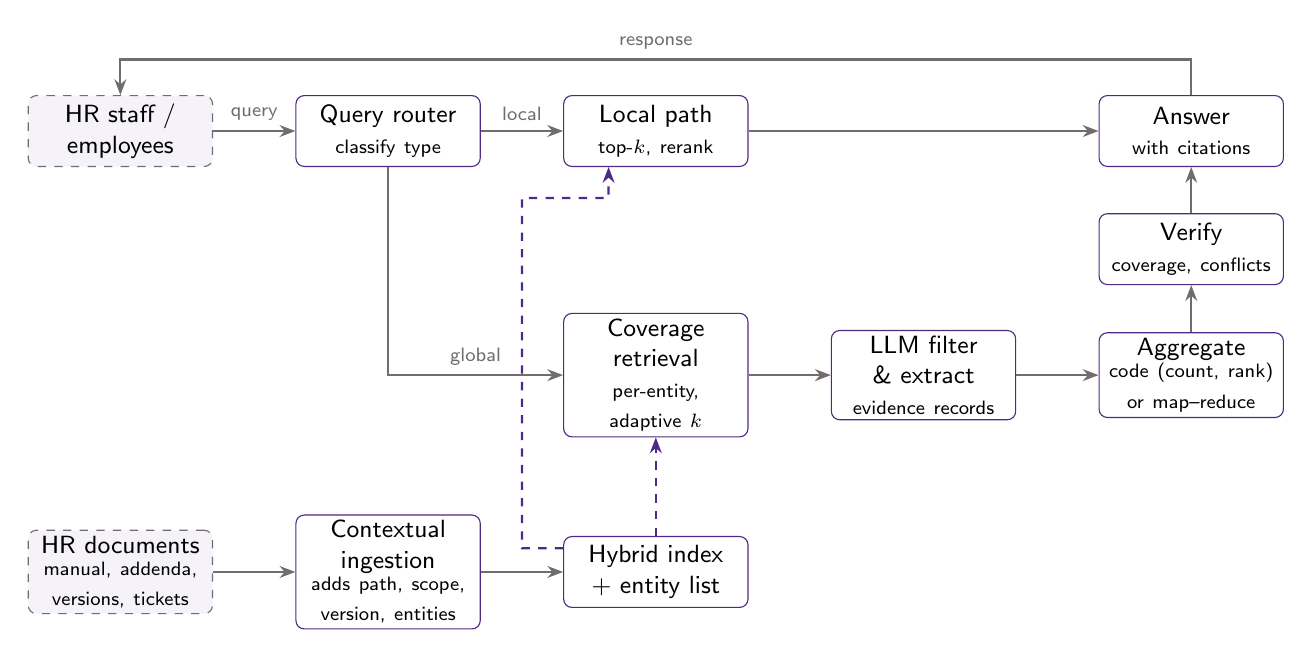
\begin{tikzpicture}[
  font=\small\sffamily,
  box/.style={draw=NUPurple, rounded corners=3pt, fill=white, align=center,
              minimum height=9mm, text width=22mm, inner sep=2pt},
  ext/.style={draw=NUGrey, dashed, rounded corners=3pt, fill=CodeBG,
              align=center, minimum height=9mm, text width=22mm, inner sep=2pt},
  arr/.style={-{Stealth[length=2mm]}, draw=NUGrey, thick},
  ret/.style={-{Stealth[length=2mm]}, draw=NUPurple, thick, dashed},
  lbl/.style={font=\scriptsize\sffamily, text=NUGrey}
]
  % row 1: user, router, local path, answer
  \node[ext] (user)   at (0,2.6)     {HR staff /\\ employees};
  \node[box] (router) at (3.4,2.6)   {Query router\\\scriptsize classify type};
  \node[box] (local)  at (6.8,2.6)   {Local path\\\scriptsize top-$k$, rerank};
  \node[box] (answer) at (13.6,2.6)  {Answer\\\scriptsize with citations};
  % row 2: global path
  \node[box] (cover)  at (6.8,-0.5)  {Coverage\\ retrieval\\\scriptsize per-entity, adaptive $k$};
  \node[box] (filter) at (10.2,-0.5) {LLM filter\\ \& extract\\\scriptsize evidence records};
  \node[box] (agg)    at (13.6,-0.5) {Aggregate\\\scriptsize code (count, rank)\\ or map--reduce};
  \node[box] (verify) at (13.6,1.1)  {Verify\\\scriptsize coverage, conflicts};
  % row 3: ingestion
  \node[ext] (docs)   at (0,-3.0)    {HR documents\\\scriptsize manual, addenda,\\ versions, tickets};
  \node[box] (ingest) at (3.4,-3.0)  {Contextual\\ ingestion\\\scriptsize adds path, scope,\\ version, entities};
  \node[box] (index)  at (6.8,-3.0)  {Hybrid index\\ + entity list};

  % query flow
  \draw[arr] (user) -- node[lbl, above]{query} (router);
  \draw[arr] (router) -- node[lbl, above]{local} (local);
  \draw[arr] (router.south) |- node[lbl, pos=0.75, above]{global} (cover.west);
  \draw[arr] (local) -- (answer);
  \draw[arr] (cover) -- (filter);
  \draw[arr] (filter) -- (agg);
  \draw[arr] (agg) -- (verify);
  \draw[arr] (verify) -- (answer);
  \draw[arr] (answer.north) -- ++(0,0.45) -| node[lbl, pos=0.25, above]{response} (user.north);
  % ingestion flow
  \draw[arr] (docs) -- (ingest);
  \draw[arr] (ingest) -- (index);
  % retrieval from the index (dashed)
  \draw[ret] (index) -- (cover);
  \draw[ret] ([yshift=3mm]index.west) -- (5.1,-2.7) -- (5.1,1.75) -| ([xshift=-6mm]local.south);
\end{tikzpicture}
\caption{Context-level architecture of the proposed LensRAG method. Dashed
arrows show retrieval from the context-enriched index; no SQL schema is built
over the corpus.}
\label{fig:context-arch}
\end{figure}

\FloatBarrier   % keep Figures 1.1 and 1.2 inside Section 1.1.1
\section{Problem Statement}
\label{sec:problem}

Standard RAG performs poorly when responding to an aggregation or a corpus-level query -- those that
require reasoning over entire corpus rather than responding from top-ranked chunks. Query responses from
standard RAG may be factually incorrect on aggregation queries, highlighting the need for effective and
evidence-based interventions. Although multiple research projects have attempted to solve this problem,
there is still an opportunity to address and measurably bridge the gaps. This project investigates approaches
to solve this problem, and we aim to improve the responses to aggregation queries on baselined datasets,
paving the way for further research in this area.

To address this problem, the project uses the enterprise HR domain as its baselined dataset. We build
an HR policy corpus for a fictional multinational, BragsLabs.
It consists of a 47-chapter policy manual with ten country addenda, extended with earlier policy versions
and related documents. On this corpus we create a set of specific and aggregation queries with verifiable
answers. We then measure how standard RAG responds to them, which gives the baseline. Next, we design
an approach that routes each query to a suitable strategy, gathers evidence from across the whole corpus
rather than only from top-ranked chunks, and computes aggregate answers exactly. Finally, we evaluate the
improvement in responses to aggregation queries against this baseline. Although the evaluation uses HR
documents, the approach avoids a fixed, domain-specific schema, so it can be applied to other document
collections and support further research in this area

\section{Research Questions and Hypotheses}
\label{sec:rq}

\begin{enumerate}[label=\textbf{RQ\arabic*.}]
  \item How well do standard RAG and long-context prompting answer global
  questions (counting, extremum, sorting, top-$k$, filtering, themes and
  sentiment) over an enterprise HR policy corpus, compared with local
  questions?
  \item Does context-enriched, coverage-oriented retrieval with query-time
  aggregation answer global questions more accurately than standard RAG,
  long-context prompting and a GlobalRAG-style baseline, and at what cost in
  tokens and latency?
  \item Can explicit verification steps detect incomplete answers and
  conflicts between policy sections or versions?
\end{enumerate}

\noindent The corresponding hypotheses are:
\begin{enumerate}[label=\textbf{H\arabic*.}]
  \item Standard top-$k$ RAG scores significantly lower on global questions
  than on local questions. Long-context prompting narrows the gap when the
  whole corpus fits in the context window, but degrades as the corpus is
  scaled beyond it.
  \item The routed pipeline achieves higher set-level F1 and exact-match accuracy on global questions than all
baselines, without reducing accuracy on local questions.
  \item Completeness and conflict checks flag a majority of incomplete or
  conflicting answers with a low false-alarm rate.
\end{enumerate}

\section{Scope and Assumptions}
\label{sec:scope}

\begin{itemize}
  \item \textbf{Corpus.} The core corpus is a single fictional company's HR
  policy manual (version 3.0, effective 1 November 2026): 47 chapters, about
  475 sections, about 41{,}000 words (roughly 55{,}000 tokens) and about 130
  tables. Chapters 1--35 cover global policies, Chapter 36 cross-border
  rules, Chapter 37 country comparison tables and Chapters 38--47 addenda for
  ten countries. Using a fictional company avoids confidentiality and
  personal-data issues.
  \item \textbf{Corpus scaling.} Because the manual alone fits in current
  long-context windows, the corpus is extended with earlier versions (v1.0
  and v2.0) and related documents such as circulars and synthetic helpdesk
  tickets, grievances and exit notes, so that the effect of corpus size can
  be measured.
  \item \textbf{Shortcut control.} Chapter 37 already aggregates many
  cross-country comparisons, which would turn global questions into local
  ones. It is excluded from the retrieval corpus and used only to check
  gold answers.

  \item \textbf{Out of scope.} Multimodal content (images, scanned
  handwriting), real employee data, multilingual documents and production
  deployment.
\end{itemize}

\section{Contributions}
\label{sec:contrib}

\begin{itemize}
  \item \textbf{Benchmark:} an HR-policy global QA test set covering local,
  counting, extremum, sorting, top-$k$, filtering, comparison, theme,
  sentiment and conflict-detection questions, with ground truth derived
  independently of the systems under test.
  \item \textbf{Method:} LensRAG, a schema-free global RAG method that
  enriches chunks with document context before embedding, retrieves for
  coverage, aggregates in code at query time and verifies completeness and
  consistency.
  \item \textbf{Empirical findings:} a comparison of standard RAG,
  long-context prompting and the proposed method on retrieval recall,
  answer accuracy, cost and latency, across three corpus sizes. On the
  largest corpus, LensRAG roughly doubles the evidence that reaches the
  generator (global recall 0.71 versus 0.36) at 0.3\% of the context of
  full-corpus prompting. With local 3B--32B models this did not raise exact
  match on global questions (0.28 for both), and it lowered local accuracy
  (Chapter~\ref{ch:results}).
  \item \textbf{Practitioner guidance:} recommendations on when global
  questions need more than standard RAG, and which strategy suits which
  question type.
\end{itemize}

\section{Report Organisation}
\label{sec:organisation}

Chapter~\ref{ch:related} reviews background and related work on RAG,
agentic and structured RAG, corpus-level aggregation and LLM-based document
analytics, and identifies the gaps this project addresses. Chapter~3
describes the methodology: corpus construction, test-set design, system
architecture and evaluation protocol. Chapter~4 covers implementation.
Chapter~5 presents results, ablations, cost--performance trade-offs and
error analysis. Chapter~6 discusses implications, limitations and ethical
considerations, and Chapter~7 concludes with future work.


%=====================================================================
%  Chapter 2 — Background and Related Work
%  Aligned with Chapter 1 (LensRAG). Requires references.bib (natbib).
%=====================================================================
\chapter{Background and Related Work}
\label{ch:related}

This chapter reviews the background needed to follow the proposed method and
the prior work it builds on. Section~\ref{sec:foundations} introduces RAG,
its known limitations and the distinction between local and global
(aggregation) queries. Section~\ref{sec:prior} groups prior work by its
principal contribution and relates each group to the design choices made in
LensRAG (Section~\ref{sec:approach}): how the corpus is organised and
partitioned, how chunks are contextualised, how retrieval achieves coverage,
how answers are aggregated, and how evidence is checked. The groups are not
mutually exclusive, since several systems combine hierarchy, graph structure,
retrieval control and evidence assessment. Section~\ref{sec:synthesis}
compares the groups, Section~\ref{sec:gap} identifies the gaps this project
addresses, and Section~\ref{sec:positioning} positions the proposed method.

\section{Foundations}
\label{sec:foundations}

\subsection{Retrieval-Augmented Generation}
Retrieval-augmented generation (RAG) couples a parametric language model with
a non-parametric document store. A retriever selects passages relevant to the
query, and the LLM model conditions its answer on them. The original
formulation combined a neural retriever with a sequence-to-sequence generator
and explored two variants, RAG-Sequence and RAG-Token, establishing the
principle that generation can be conditioned on external evidence
retrieved rather than relying entirely on parametric knowledge \citep{lewis2020rag}.
RAG has since become the default way to ground large language models (LLMs)
in private or frequently changing knowledge, because it reduces hallucination
and allows sources to be updated without retraining
\citep{gao2023ragsurvey}. A typical pipeline splits documents into fixed-size
chunks, embeds them, retrieves the top-$k$ most similar chunks for a query,
and passes them to the LLM as context. The corpus-level approaches reviewed in
this chapter extend that principle by changing how the external collection is
structured, searched, and checked.

\subsection{Known Limitations of Standard RAG}
Practitioner and survey studies have cataloged recurring failure points in
this pipeline \citep{barnett2024sevenfailure,gao2023ragsurvey}. On the
retrieval side, relevant content may be missed due to vocabulary
mismatch, poor fragment boundaries that separate conditions from their
exceptions, or a cut-off point $k$ too small. A chunk also loses the
context of the document it came from: a clause such as ``this applies for
10 days'' no longer says which country, policy or version it belongs to. On
the generation side, models may ignore or misread retrieved evidence, are
sensitive to where evidence appears in a long context
\citep{liu2024lostmiddle}, and rarely flag contradictions between sources.
These limitations are tolerable for \emph{local} questions, whose answers lie
in one or a few passages. They become decisive for \emph{global} questions,
whose answers depend on evidence spread across the whole corpus.

\subsection{Local versus Global Queries}
\citet{edge2024graphrag} first drew the distinction between local and global
questions, observing that standard RAG fails on corpus-wide questions such as
``What are the main themes in this dataset?'', which are closer to
query-focused summarisation than to retrieval. \citet{luo2025globalrag}
sharpen the definition: \emph{global RAG} requires aggregating and analysing
information across an entire collection, as in counting, extremum, sorting
and top-$k$ queries. In this setting a retriever must find \emph{all}
relevant items rather than the \emph{most} relevant ones, and the answer must
be computed exactly rather than paraphrased. This report uses the term
\emph{aggregation queries} for both kinds: those that need an exact
computation (count, extremum, rank, top-$k$, filter) and those that need a
corpus-wide summary (themes, sentiment shift).

\section{Prior Work}
\label{sec:prior}

\subsection{Advanced and Adaptive RAG}
A first line of work improves the retrieve-then-generate loop itself. FLARE
triggers retrieval when generation confidence is low \citep{jiang2023flare},
IRCoT interleaves retrieval with chain-of-thought reasoning for multi-hop
questions \citep{trivedi2023ircot}, and Self-RAG learns to decide whether
external retrieval is needed at all \citep{asai2024selfrag}. These methods
make retrieval less dependent on a single fixed decision at the start of the
pipeline and improve robustness for local and multi-hop questions. They still
assume that a small evidence set is sufficient, so they do not address the
completeness requirement of aggregation queries. Their evidence-assessment
mechanisms are discussed in Section~\ref{sec:verification}.

\subsection{Corpus Organisation, Chunking and Context-Enriched Embeddings}
\label{sec:organisation-rw}
Because fixed-size chunking strips each passage of its surrounding context,
several methods restore that context or organise the corpus into levels of
abstraction. Late chunking embeds the full document with a long-context
embedding model and only then pools token embeddings into chunk vectors, so
each chunk vector reflects the document around it
\citep{gunther2024latechunking}. RAPTOR groups semantically related text
units, summarises each group and repeats the process to build a tree of
increasingly broad summaries, so retrieval can draw on detailed passages or
on summaries that represent a wider context \citep{sarthi2024raptor}. RAPTOR
established an influential approach to multi-resolution retrieval, but a tree
does not by itself express every relationship between branches or between
separate documents. $\Psi$-RAG applies the same idea across documents: its tree of abstracts can
be restructured by merging and collapsing nodes, and an agent decides at each
step whether to read a broad abstract or descend to detailed text
\citep{zhao2026psirag}. The central issue it addresses is
granularity: a system needs a compact view of the corpus for orientation, but
must be able to return to the underlying evidence when a question requires
detail.

Chunking choices also matter empirically. \citet{maharjan2026chunking}
evaluate RAG configurations on public-health policy documents, comparing a
language model without retrieval, a basic semantic-search pipeline and a
pipeline that adds cross-encoder reranking. They report higher faithfulness
with retrieval and a further improvement with reranking, and show that
retrieval quality depends on linked choices, including how source documents
are segmented and how candidates are ordered. This result is directly
relevant to the policy domain studied here. LensRAG follows the same
structure-aware view of chunking: it splits documents along their section
structure, keeps tables whole, and prepends a structured contextual header
(document, section path, scope, version and entities) to each chunk before
embedding, so that every relevant clause remains findable and attributable to
the right entity during aggregation.

\subsection{Corpus Partitioning and Domain Scoping}
\label{sec:partitioning}
Semantic similarity is not always an adequate basis for organising a large
collection. \citet{maio2026olap} approach corpus organisation through
concepts from analytical data management: their position paper adapts the
Dimensional Fact Model, using dimensions such as time and organisational
context to partition the corpus and route retrieval. This perspective suits
enterprise collections, where a useful search boundary may be defined by
business unit, reporting period or another operational attribute rather than
by topic alone. \citet{subedi2026dilution} study what happens as an
index grows: passages that are close in meaning but belong to the wrong
context crowd out the right ones, which they term \emph{vector search
dilution}, and restricting search to the relevant domain through metadata
reduces the problem. Both studies imply that increasing corpus size does not automatically
improve retrieval, and that search boundaries may need to reflect domain or
organisational context. In LensRAG, the scope, version and entity fields of
each chunk header serve this purpose: per-entity sub-queries are restricted
to the relevant country, policy version or document type, which limits
dilution as the corpus grows from the core manual to its extended versions.

\subsection{Agentic RAG and Query Decomposition}
A further line embeds autonomous agents in the pipeline. Agents decompose a
query into sub-tasks, choose tools, retrieve iteratively and verify
intermediate results \citep{singh2025agenticrag}. Recent systematisation
work formalises agentic RAG as a partially observable sequential decision
process and argues that static generation metrics are insufficient to
evaluate it \citep{mishra2026sokagenticrag}. Reinforcement learning has also
been used to train models to interleave reasoning with search calls
\citep{jin2025searchr1}.

Decomposition is the agentic step most relevant to aggregation. HiRAG
separates the work into decomposition, definition, retrieval, filtering and
summarisation, combines document-level sparse retrieval with chunk-level
dense retrieval, and uses a rethink step to trigger another retrieval attempt
when the evidence is insufficient \citep{zhang2024hirag}.
\citet{ammann2025decomposition} first separate a complex question into
smaller information needs, retrieve passages for each sub-question, merge the
candidates and apply cross-encoder reranking; this makes implicit evidence
requirements visible and improves coverage, at the cost of more retrieval
operations and a larger candidate set. \citet{petcu2026exploration} treat
decomposition as a balance between exploring for additional evidence and
exploiting what has already been found, using feedback about document
usefulness to spend more effort on unresolved sub-questions. SParC-RAG
coordinates sequential refinement and parallel exploration of distinct
sub-queries over a shared global context, aiming to keep the benefits of
exploration without letting the evidence set grow without control
\citep{yang2026sparcrag}. These studies show the value of focused,
decomposed retrieval, but each additional query, tool call or reasoning step
increases latency and cost. LensRAG uses a restricted form of decomposition:
one sub-query per relevant entity, taken from an entity list built at
ingestion, which keeps the number of sub-queries bounded and makes coverage
checkable.

\subsection{Retrieval Quality, Coverage and Evidence Selection}
Several studies argue that retrieving more is not the same as retrieving
well. \citet{zheng2026migrascope} argue that standard scores such as recall and
Mean Reciprocal Rank say little about what each retriever adds when several
are combined. Their benchmark, MIGRASCOPE, uses mutual-information measures
to estimate how much a retriever overlaps with, complements or adds to the
others; in their experiments dissimilar retrievers add complementary
evidence, whereas closely related ones largely repeat each other. \citet{peng2026neocorrag} show that
high recall does not necessarily produce accurate answers, introduce the
Recall Conversion Rate, and use evidence chains in NeocorRAG to remove
distractions and make connections between facts explicit. TRACE converts
retrieved documents into a knowledge graph and builds reasoning chains step by
step, with a triple ranker proposing candidates and an LLM selecting the next
triple \citep{fang2024trace}. On HotpotQA, 2WikiMultiHopQA and MuSiQue it
improves average exact-match accuracy by 14.03 percentage points over using
all retrieved documents, with much shorter answer context, although it relies
on title-centred Wikipedia graph extraction and does not directly evaluate
chain quality.

For aggregation queries, coverage becomes the primary requirement.
PluriHopRAG is designed for questions where missing a single relevant
document makes the answer wrong and where many near-miss documents are
present \citep{sveistrys2025plurihop}. Instead of stopping at the top-$k$, it
asks a sub-question of each document and uses a cross-encoder to drop
irrelevant ones before the LLM reasons over the rest. LensRAG follows the same principle of
retrieving until no new relevant evidence appears, combines keyword and dense
retrieval as complementary signals in the sense of
\citet{zheng2026migrascope}, and applies an LLM filter that keeps only
passages satisfying the query condition, which addresses the precision
concerns raised by \citet{peng2026neocorrag}.

\subsection{Structured and Graph-Based RAG}
Another line makes relationships within the collection explicit. GraphRAG
extracts entities and relationships, detects hierarchical communities,
pre-computes community summaries and combines community-level partial answers
into a global response with a map--reduce step, shifting the retrieval target
from isolated passages to connected groups of concepts
\citep{edge2024graphrag}. The trade-off is the processing needed to extract
entities, build the graph and generate summaries. LeanRAG points out that
community summaries can end up isolated from one another even when their
topics overlap, a problem its authors call \emph{semantic islands}. It
therefore adds explicit links between summary-level concepts and retrieves
from the fine-grained entities upwards through these links
\citep{zhang2026leanrag}. HippoRAG uses a graph as a
memory structure and applies personalised PageRank to find connected
knowledge, which helps when a question requires following a chain of
associations \citep{gutierrez2024hipporag,gutierrez2025hipporag2}. LightRAG
combines graph-based organisation with vector retrieval, supports both
entity-level and theme-level searches, and supports incremental updates
\citep{guo2024lightrag}. Knowledge Graph Prompting represents both document
content and document structure, such as pages and tables, as graph nodes and
uses LLM-guided traversal to select material for multi-document question
answering, showing that useful context may lie in a passage's position and
relationship to other document components \citep{wang2024kgp}.
\citet{jia2026heterograph} extend graph RAG to heterogeneous academic graphs
of authors, papers and venues, with agents for query-aware retrieval,
evidence expansion and graph-grounded verification.

Graph retrieval is not universally better, however. \citet{han2026ragvsgraphrag}
compare conventional RAG and GraphRAG on factual questions, multi-hop
reasoning and query-focused summarisation, and find that passage-based RAG
often fits narrowly defined factual lookups, while graph-oriented methods help
when the task depends on broader connections; retrieval should therefore be
selected according to the question. StructRAG follows this logic by routing
each task to the most suitable structure type (for example a table, graph or
catalogue), converting the documents into that structure at inference time
and answering from it, with the largest gains when information is highly
scattered \citep{li2025structrag}.

Structured RAG (S-RAG) is the closest structured approach to aggregation: during
indexing it turns the documents into database records, and at query time it
answers questions by generating SQL over those records
\citep{koshorek2025srag}.
This gives exact answers when the schema covers the question, but requires
the schema to be defined and populated in advance. Summary-based methods such
as GraphRAG suit thematic questions but lose exact values during
summarisation. LensRAG takes elements of both: like StructRAG and
\citet{han2026ragvsgraphrag}, it routes by query type; like GraphRAG, it uses
map--reduce for theme and sentiment queries; but unlike S-RAG, it builds no
schema or database over the corpus.

\subsection{Knowledge Refinement and Structured Reasoning}
A relevant passage can still contain details that do not help answer the
current question, so other work refines retrieved knowledge before
generation. RankCoT combines ranking signals with reasoning-based
summarisation, using preference training and self-reflection to produce
concise, relevant evidence \citep{wu2025rankcot}. CoT-RAG combines
knowledge-graph-guided reasoning, case-aware retrieval and structured
pseudo-program prompts, using intermediate reasoning steps to organise the
information need and retrieve relevant cases for each part of the task
\citep{li2025cotrag}. These approaches improve how evidence is used, but
depend respectively on reliable training examples and on retrieved cases and
graph relationships that adequately support the answer. LensRAG instead
refines evidence into short query-time records of (entity, value, evidence
span), which need no training and keep every value traceable to its source.

\subsection{Evidence Verification and Conflict Handling}
\label{sec:verification}
A dependable system must recognise weak or conflicting evidence rather than
treating every retrieved passage as trustworthy. Self-RAG learns, through
reflection tokens, to assess the relevance of retrieved passages and to judge
whether a generated response is supported by them, making evidence assessment
part of generation rather than an afterthought \citep{asai2024selfrag}.
Corrective RAG (CRAG) adds a lightweight retrieval evaluator that grades the
retrieved results and, when they are unreliable or insufficient, refines them
or consults additional sources before generating an answer
\citep{yan2024crag}. EG-RAG goes a step further and builds a graph over
the evidence itself \citep{hong2026egrag}: pairs of relevant sentences are
labelled by a natural language inference model as agreeing, disagreeing or
unrelated, and the resulting weighted links let the system tell
corroboration apart from conflict. This is particularly pertinent to large corpora, where
documents may report incompatible claims or reflect different versions of the
same information. Policy corpora are a clear case: a value may differ between
a global chapter, a country addendum and an older policy version. LensRAG's
verification step addresses this by checking completeness against the entity
list, flagging conflicting values from different sections or versions, and
confirming that every statement in the answer is backed by an evidence span.

\subsection{Corpus-Level Aggregation: Benchmarks and Methods}
The work closest to this project explicitly targets aggregation over text.
\citet{luo2025globalrag} introduce GlobalQA, a benchmark of counting,
extremum, sorting and top-$k$ queries that require evidence from many
documents. On this benchmark the best existing RAG baseline scores only
1.51 F1. Their own system, GlobalRAG, keeps documents intact as retrieval
units, removes irrelevant documents with an LLM-based filter and leaves the
final counting or ranking to symbolic tools; with Qwen2.5-14B it reaches
6.63 F1. The same group's MARAG-R1 moves beyond a
single retriever and a fixed top-$k$ result set: an LLM agent coordinates
semantic search, keyword search, document filtering and result aggregation,
and supervised fine-tuning followed by reinforcement learning trains its
decisions about which tools to invoke over multiple steps
\citep{luo2025maragr1}. \citet{zhu2026aggbench} treat aggregation as a task in which the answer must
be grounded in a fixed corpus and every qualifying entity must be found. Their
benchmark, AGGBench, is drawn from finance reports and research papers and
checked by human annotators, and their DFA baseline splits the work into
three stages (resolving what the query refers to, filtering candidates, then
aggregating), which finds more of the required evidence than RAG and agentic
baselines. CorpusQA pushes the corpus size to 10 million tokens; its answers are
produced by code rather than annotators, by turning documents into tables and
running SQL over them \citep{lu2026corpusqa}. It also finds that long-context
models lose accuracy quickly as the corpus grows. Together
these works establish that aggregation queries are largely unsolved, and that
completeness of evidence and exact computation are the central difficulties.
LensRAG shares GlobalRAG's filter-then-compute design and DFA's emphasis on
completeness; unlike MARAG-R1, it requires no model training, and it adds
context-enriched indexing and explicit verification.

\subsection{LLM-Powered Analytics over Unstructured Documents}
The database community approaches the same problem as query processing over
documents. Early work such as EVAPORATE extracts structured views from
semi-structured documents with LLMs \citep{arora2023evaporate}. LOTUS
defines \emph{semantic operators}: relational operations such as filter,
join, rank and aggregate whose conditions are written in natural language and
evaluated by an LLM, so that they can be chained like database queries
\citep{patel2025lotus}. Its authors note that RAG and Text-to-SQL suit only
analyses whose evidence fits in one model call. DocETL optimises LLM document-processing
pipelines through agent-driven rewrites \citep{shankar2025docetl}, and
Palimpzest provides cost-aware declarative optimisation of such pipelines
\citep{liu2025palimpzest}. Aryn combines layout-aware parsing with Luna, a
planner that translates natural-language questions into inspectable query
plans, and reports better accuracy than RAG on analytic queries over
accident reports \citep{anderson2025aryn}. UDA-Bench provides a large
benchmark for this setting, with over 100{,}000 documents and 240 queries
spanning selection, filtering, aggregation and joins
\citep{deng2026udabench}. This literature shows that LLM extraction followed
by exact computation outperforms free-text reasoning for analytic queries.
LensRAG adopts that principle but keeps it lightweight: values are extracted
only for the passages a query needs, held as temporary records and computed
in code, rather than materialised as tables over the whole corpus.

\subsection{Long-Context Models as an Alternative}
Million-token context windows raise the question of whether retrieval is
needed at all for small corpora. Evidence suggests that long context does not
remove the problem: models under-use information in the middle of long
inputs \citep{liu2024lostmiddle}, and on corpus-level analysis tasks
accuracy falls substantially as context length grows from 128K to 1M tokens
\citep{lu2026corpusqa}. StructRAG likewise outperforms a long-context
baseline on knowledge-intensive tasks \citep{li2025structrag}. Long-context
prompting therefore remains an essential \emph{baseline}, particularly when a
corpus fits in the window, as the core BragsLabs policy manual does, but not a
general solution.

\section{Comparative Discussion}
\label{sec:synthesis}

Taken together, the studies suggest that corpus-level RAG is not a single
retrieval technique but a set of interdependent design choices. A first group
changes how information is organised before a question is asked: RAPTOR,
$\Psi$-RAG and HiRAG give access to information at different levels of
abstraction, LeanRAG links related summaries, and OLAP-inspired partitioning
and domain scoping define organisational boundaries for retrieval. A second
group makes relationships explicit: GraphRAG, HippoRAG, LightRAG, Knowledge
Graph Prompting and heterogeneous graph RAG connect entities, passages or
document components, although the comparison by \citet{han2026ragvsgraphrag}
cautions against treating graph retrieval as a universal replacement for
passage search. A third group decides how retrieval should proceed:
decomposition, exploration--exploitation, SParC-RAG and multi-tool agents such
as MARAG-R1 aim to broaden coverage where it is needed. A fourth group
assesses the evidence passed to the generator: reranking and
information-theoretic evaluation judge retrieved candidates, RankCoT and
NeocorRAG refine how information is represented, and Self-RAG, CRAG and
EG-RAG detect unreliable or conflicting evidence. Finally, aggregation-focused
work (GlobalRAG, DFA, CorpusQA and database-style systems) shows that exact
answers require exhaustive evidence and computation outside the LLM.

These choices involve trade-offs. Hierarchies provide compact navigation but
may obscure links between branches. Graphs make relationships explicit but
require construction and maintenance. Adaptive agents can broaden or refine a
search but consume more time and computation. Evidence filtering reduces
noise, yet overly aggressive filtering risks discarding a passage that is
necessary in combination with others. A practical architecture therefore
needs to select and coordinate these capabilities according to the question,
the corpus and the required level of assurance, which is the approach taken by
LensRAG's query router.

\section{Gap Analysis}
\label{sec:gap}

Table~\ref{tab:gap} summarises how representative prior work relates to the
requirements of this project. Five gaps stand out.

\begin{enumerate}
  \item \textbf{Domain.} Existing aggregation benchmarks are built from
  encyclopaedic, academic, financial or incident-report corpora. Policy
  documents have been studied for local question answering
  \citep{maharjan2026chunking}, but to our knowledge no work evaluates
  aggregation queries over enterprise policy, where answers depend on
  jurisdiction, versioning, exceptions and cross-references between chapters.
  \item \textbf{Exact aggregation without SQL.} Methods that compute exact
  answers usually build tables or a schema over the corpus in advance
  \citep{koshorek2025srag,lu2026corpusqa,patel2025lotus}, whereas schema-free
  methods compute less reliably. Few works obtain exact counts and rankings
  from a plain text and vector index, with structure created only at query
  time.
  \item \textbf{Context and scope at indexing.} Context-enriched embeddings
  \citep{gunther2024latechunking} and metadata-based partitioning
  \citep{maio2026olap,subedi2026dilution} have been studied separately,
  mainly for local retrieval. They have not been combined as a means of
  making every relevant clause findable, correctly scoped and attributable
  for aggregation queries.
  \item \textbf{Evidence completeness and conflicts across versions.}
  Passage relevance does not establish that every entity in an aggregation
  has been covered. Conflict-aware methods such as EG-RAG
  \citep{hong2026egrag} detect contradictions between statements, but few
  systems verify completeness or distinguish a true conflict from a
  legitimate policy update across versions.
  \item \textbf{Consistent evaluation.} Prior studies use different tasks
  and measures. Few report aggregation accuracy, retrieval recall,
  faithfulness, cost and latency together, or test both local lookup and
  corpus-level aggregation on the same corpus.
\end{enumerate}

\begin{table}[htbp]
\centering\small
\caption{Positioning of representative prior work against the requirements
of this project. Entries summarise each work's primary focus as described by
its authors.}
\label{tab:gap}
\begin{tabularx}{\textwidth}{@{}l X X X@{}}
\toprule
\textbf{Work} & \textbf{Target queries} & \textbf{How answers are computed} & \textbf{Corpus / domain} \\
\midrule
GraphRAG \citep{edge2024graphrag} & Global, thematic sense-making & Map--reduce over community summaries & Podcasts, news \\
StructRAG \citep{li2025structrag} & Knowledge-intensive, scattered & Task-specific structures built at inference & General QA benchmarks \\
S-RAG \citep{koshorek2025srag} & Aggregative questions & Schema built at ingestion; SQL queries & Aggregative QA datasets \\
GlobalRAG \citep{luo2025globalrag} & Count, extremum, sort, top-$k$ & LLM filtering + symbolic aggregation & Encyclopaedic corpus \\
MARAG-R1 \citep{luo2025maragr1} & Corpus-level QA & RL-trained multi-tool retrieval agent & GlobalQA \\
DFA / AGGBench \citep{zhu2026aggbench} & Entity-level aggregation, completeness & Disambiguate--filter--aggregate agent & Finance reports, papers \\
PluriHopRAG \citep{sveistrys2025plurihop} & Exhaustive, recall-sensitive QA & Per-document sub-questions + cross-encoder filter & Distractor-rich corpora \\
EG-RAG \citep{hong2026egrag} & Multi-document reasoning & NLI-based evidence graph (support/contradict) & Multi-document QA \\
LOTUS \citep{patel2025lotus} & Bulk semantic analytics & Declarative semantic operators & Various \\
\midrule
\textbf{LensRAG (this project)} & Local and aggregation queries, incl.\ themes, sentiment and conflicts & Context-enriched, scoped embeddings; per-entity coverage retrieval; query-time extraction; computation in code or map--reduce; verification; no SQL & Enterprise HR policy (multi-country, multi-version) \\
\bottomrule
\end{tabularx}
\end{table}

\section{Positioning of This Work}
\label{sec:positioning}

This project extends corpus-level aggregation
\citep{luo2025globalrag,zhu2026aggbench} to a new domain, enterprise HR
policy, through the LensRAG method described in Section~\ref{sec:approach}.
Each of its components builds on established work: structure-aware,
context-enriched chunk embeddings
\citep{gunther2024latechunking,maharjan2026chunking}, metadata scoping of
retrieval \citep{maio2026olap,subedi2026dilution}, query routing by type
\citep{li2025structrag,han2026ragvsgraphrag}, entity-level decomposition and
coverage-oriented retrieval
\citep{ammann2025decomposition,sveistrys2025plurihop,yang2026sparcrag}, LLM
filtering followed by symbolic aggregation \citep{luo2025globalrag},
map--reduce summarisation for thematic queries \citep{edge2024graphrag}, and
evidence verification with conflict detection
\citep{yan2024crag,hong2026egrag}. To our knowledge, the combination has not
been evaluated on aggregation queries, and it differs from S-RAG
\citep{koshorek2025srag} and database-style systems \citep{patel2025lotus} in
that no schema or SQL database is built over the corpus, and from MARAG-R1
\citep{luo2025maragr1} in that it requires no model training. Following
\citet{lu2026corpusqa}, ground truth for aggregation queries is derived
independently of the systems under test so that results are verifiable, and
a long-context baseline is included because the core policy manual fits
within current context windows. The evaluation reports aggregation accuracy,
retrieval recall, faithfulness, cost and latency together, and adds
completeness and conflict-detection measures that prior benchmarks do not
report.

\chapter{Methodology}
\label{ch:methodology}

\section{Research Design}
\label{sec:design}

The study is \emph{experimental}, within a design-science frame. The artefact
is LensRAG (Section~\ref{sec:approach}). It is evaluated in controlled,
repeatable experiments against standard retrieval-augmented generation (RAG)
and long-context baselines on a corpus whose ground truth is known exactly.
This design was chosen for three reasons.
\begin{enumerate}
  \item The hypotheses (Section~\ref{sec:rq}) are comparative and
  quantitative, so they need paired measurements of several systems on the
  same questions rather than a survey or case study.
  \item Aggregation answers (counts, rankings, shares) can only be scored
  objectively if the true answer is computed independently of the systems
  under test \citep{lu2026corpusqa}. A synthetic corpus generated from a
  ledger provides this (Section~\ref{sec:data}).
  \item Corpus size is the main independent variable for H1, so the same
  questions must be answerable at several corpus sizes. The corpus is
  therefore built in three nested tiers.
\end{enumerate}

Each experiment has three factors: the \emph{method} (standard top-$k$ RAG,
long-context prompting, LensRAG and its variants), the \emph{corpus tier}
(S, M, L) and the \emph{question scope} (local or global). Measurements are
taken at two levels:
\begin{itemize}
  \item \textbf{Retrieval level:} do the gold evidence documents reach the
  context the generator reads? This is deterministic and model-free, and was
  run on all three tiers.
  \item \textbf{Answer level:} is the final answer correct? This needs a
  generator LLM, and was run on tier L, the largest and hardest tier.
\end{itemize}

\section{System Architecture}
\label{sec:architecture}

Figure~\ref{fig:context-arch} shows the context-level architecture and
Figure~\ref{fig:pipeline} the query pipeline. The implementation follows the
nine steps of Section~\ref{sec:approach}:
\begin{itemize}
  \item steps 1--2 (ingestion and indexing) run once, offline;
  \item steps 3--9 run per question.
\end{itemize}
The rest of this section describes each component and why it was chosen. The
models are listed in Table~\ref{tab:models} (candidates) and
Table~\ref{tab:used-models} (models actually used).

\paragraph{Ingestion and context enrichment (steps 1--2).}
Documents are Markdown files with YAML front matter (document id, type,
country, version, effective date, period, status). Each document is split at
its headings into sections. A section longer than 260 words is split again at
paragraph boundaries, and very long passages are cut into 260-word windows
with a 40-word overlap. Markdown tables are never split. Each chunk receives
a context header, for example:
\begin{quote}\small\ttfamily\raggedright
Document: Chapter 41. Germany addendum [POL-DE] | Type: policy | Section:
Leave | Scope: DE | Version: 3.0 | Status: current | Entities: Germany
\end{quote}
The header is embedded together with the chunk text. During ingestion an
\emph{entity inventory} is built: every country, office, policy version and
period found in the corpus, with aliases. Entity types, field mappings,
status words and record types are declared in a domain configuration file
(YAML). This keeps the method from being tied to HR; a second configuration
for a legal corpus demonstrates this. Chunks, their metadata and their
vectors are persisted in ChromaDB, so the 13{,}187-chunk tier-L index is
built once and reused.

\paragraph{Hybrid retrieval.}
Every method uses the same hybrid retriever: BM25 for exact terms (policy
names, document ids, numbers) plus a dense or TF-IDF similarity, combined by
rank fusion. Dense retrieval uses BGE-M3 \citep{chen2024bgem3}, a
multilingual embedding model that runs locally.

\paragraph{Planning and entity decomposition (steps 3--4).}
A small LLM classifies the question into one of the twelve question types and
extracts its parameters: attribute, condition, period, version and
aggregation. Entities named in the question are matched to the inventory by
lookup. An optional spaCy named-entity recogniser with fuzzy matching catches
spelling variants and possessives. For a global question with no named
entity, the scope is every inventory entity of the relevant type (for
example, all ten countries with an addendum). Superseded versions are
excluded unless the question asks about a version or a date.

\paragraph{Coverage-oriented retrieval (step 5).}
Each entity scope is searched separately. The retriever fetches one page of
five chunks per scope per round, and paging continues until a round yields no
new relevant chunk. The relevance judgement comes from one of three sources:
\begin{itemize}
  \item the LLM filter in the full pipeline;
  \item a cross-encoder in the retrieval benchmark: BGE-reranker-v2-m3, with
  a threshold calibrated on held-out questions
  (Section~\ref{sec:eval});
  \item for local questions, a reranker in place of the LLM judge.
\end{itemize}
A scope that yields no relevant evidence is recorded and later reported as a
possible gap in completeness.

\paragraph{Evidence extraction (step 6).}
A mid-size LLM reads each retrieved chunk and returns JSON evidence records.
Each record holds the entity, attribute, value, unit, version, the supporting
text span and the chunk id. Records whose span does not occur in the chunk
are discarded.

\paragraph{Computation (step 7).}
The answer is computed in one of three modes, chosen from the question type
and the number of records in scope:
\begin{itemize}
  \item \emph{Mode A, exact.} Counts, extrema, rankings, top-$k$, filters,
  sums and categorical tallies are computed in Python over the evidence
  records, never by the LLM.
  \item \emph{Mode B, estimated.} This mode handles questions over record logs
  too large to read in full (for example, 6{,}038 helpdesk tickets). LensRAG
  draws a stratified random sample of 150 records and labels each one three
  times. It reports a point estimate with a 95\% interval: Wilson intervals
  for proportions and a stratified bootstrap for means, both with a
  finite-population correction. Sentiment can be labelled with a RoBERTa
  classifier, giving soft labels.
  \item \emph{Mode C, generated.} Theme and insight questions use map--reduce.
  The reduce step is repeated five times and only claims that appear in a
  majority of runs are kept. Each claim carries its support and citations,
  and any number in the generated text that is absent from the evidence is
  flagged.
\end{itemize}

\paragraph{Verification and answer (steps 8--9).}
The verifier checks three things:
\begin{itemize}
  \item \emph{completeness:} every scope in the plan has evidence;
  \item \emph{consistency:} the same attribute does not carry different
  values in different documents. Values that differ across versions are
  resolved by version and effective date rather than reported as conflicts;
  \item \emph{provenance:} every number in the answer traces back to an
  evidence record.
\end{itemize}
An optional DeBERTa-v3-large natural-language-inference model checks each
answer sentence against focused premises built from the evidence. A strong
LLM then writes the answer with citations and any flags.

\paragraph{Model routing.}
Each LLM call names a \emph{role}: classify, extract, map, reduce, verify or
answer. A routing layer sends each role to its own model. This puts the
cheap, high-volume steps on small models, as Table~\ref{tab:models}
proposes. Providers are interchangeable: the same code runs on Claude, on
any OpenAI-compatible endpoint, or on local models served by Ollama.

\begin{table}[htbp]
\centering\small
\caption{Candidate models for each stage of the LensRAG query pipeline.
The models used in the experiments are listed in Table~\ref{tab:used-models}.}
\label{tab:models}
\setstretch{1.1}
\begin{tabularx}{\textwidth}{@{}>{\raggedright\arraybackslash}p{3.1cm} >{\raggedright\arraybackslash}X >{\raggedright\arraybackslash}X@{}}
\toprule
\textbf{Stage (model role)} & \textbf{Open-source / self-hosted} & \textbf{API / hosted} \\
\midrule
Classify query type \newline\emph{(small LLM classifier)} &
Qwen2.5-3B-Instruct or Phi-4-mini (few-shot); or a fine-tuned DeBERTa-v3 / SetFit classifier &
GPT-4o-mini, Claude Haiku, Gemini Flash \\ \addlinespace[4pt]
Search + rerank \newline\emph{(hybrid + reranker)} &
BM25 (OpenSearch / Elasticsearch) + BGE-M3 embeddings; bge-reranker-v2-m3 &
OpenAI text-embedding-3-large or Voyage embeddings; Cohere Rerank \\ \addlinespace[4pt]
Select relevant entities \newline\emph{(rules + LLM)} &
Lookup over the ingestion-time entity list + spaCy NER; small LLM fallback &
Same rules; GPT-4o-mini or Claude Haiku fallback \\ \addlinespace[4pt]
Per-entity adaptive retrieval \newline\emph{(embedder + BM25 + LLM)} &
Same hybrid index; Qwen2.5-7B-Instruct for sub-queries and stopping &
Same hybrid index; GPT-4o-mini or Claude Haiku \\ \addlinespace[4pt]
LLM filter + extract \newline\emph{(fast LLM, JSON output)} &
Qwen2.5-7B/14B-Instruct or Llama-3.1-8B-Instruct with JSON-constrained decoding (vLLM / Ollama) &
GPT-4o-mini (structured outputs); Claude Haiku (tool-use JSON) \\ \addlinespace[4pt]
Compute in code \newline\emph{(no model)} &
Python / pandas (count, max, sort, top-$k$) &
-- \\ \addlinespace[4pt]
Map--reduce summarise \newline\emph{(strong LLM)} &
Qwen2.5-72B-Instruct or Llama-3.3-70B-Instruct; optional RoBERTa sentiment classifier for per-record labels &
GPT-4o, Claude Sonnet, Gemini Pro \\ \addlinespace[4pt]
Verify evidence \newline\emph{(LLM judge + rules)} &
Rule checks (entity coverage, cross-version values); DeBERTa-v3-large NLI; Qwen2.5-14B judge &
Rule checks; GPT-4o or Claude Sonnet judge; RAGAS faithfulness \\ \addlinespace[4pt]
Generate answer \newline\emph{(strong LLM + citations)} &
Qwen2.5-72B-Instruct or Llama-3.3-70B-Instruct &
GPT-4o, Claude Sonnet, Gemini Pro \\
\bottomrule
\end{tabularx}
\end{table}

\section{Data and Benchmarks}
\label{sec:data}

\paragraph{Corpus.}
The BragsLabs HR corpus (version 1.0, built 5 November 2026) is a synthetic
document collection for a fictional multinational. It contains 500 Markdown
files and about 1.52 million words, with no real people or employee data
(Table~\ref{tab:corpus}). It contains:
\begin{itemize}
  \item three versions of the HR policy manual (v1.0, v2.0 and the current
  v3.0, with ten country addenda);
  \item 60 HR circulars, six of which announce changes effective in 2027;
  \item 30 FAQs, 14 office handbooks and 10 benefits summaries;
  \item four record logs: 6{,}038 helpdesk tickets, 1{,}697 grievance cases,
  960 exit interviews and 3{,}850 pulse-survey comments.
\end{itemize}

\paragraph{Construction.}
The corpus is generated \emph{ledger first}, by standard-library Python
scripts with a fixed seed:
\begin{enumerate}
  \item The facts are generated first and stored as JSON ledgers: every
  policy value by country and version, circulars, key events, planted
  conflicts, and every individual record with its category, date, sentiment
  label and resolution time.
  \item The documents are then rendered from the ledger with templates.
  \item A validator runs about 2{,}700 checks: that the text agrees with the
  ledger, that the planted conflicts are present, that record counts are
  correct and that every evidence id exists.
\end{enumerate}

\paragraph{Planted signals.}
The corpus contains deliberate signals for a system to find:
\begin{itemize}
  \item \emph{Events with measurable effects.} The rise from two to three
  hybrid office days on 1 April 2026 increases hybrid tickets and grievances,
  and makes exit sentiment more negative. The migration to a new expense
  module raises reimbursement volumes and resolution times.
  \item \emph{Conflicts.} Twelve conflicts are planted: an internal
  inconsistency in India sick leave, future-dated circulars, stale FAQs,
  stale handbooks and a stale benefits summary. Legitimate version updates
  are included as negative controls.
\end{itemize}

\paragraph{Tiers and shortcut control.}
The tiers are nested (Table~\ref{tab:corpus}). Five documents that
pre-aggregate answers are flagged \texttt{retrieval\_exclude} and are never
indexed: the country-comparison chapter in v2.0 and v3.0, the change log and
the two annual reports. They are used only to check gold answers.

\begin{table}[htbp]
\centering\small
\caption{Corpus tiers. Tokens counted with \texttt{tiktoken cl100k\_base};
chunks after context-enriched chunking.}
\label{tab:corpus}
\begin{tabular}{@{}llrrrr@{}}
\toprule
Tier & Contents & Documents & Words & Tokens & Chunks \\
\midrule
S & Manual v3.0 & 46 & 45{,}069 & 59{,}912 & 580 \\
M & S + v1.0, v2.0, circulars, FAQs, handbooks, benefits & 245 & 250{,}423 & 335{,}180 & 3{,}441 \\
L & M + tickets, grievances, exit notes, surveys & 495 & 1{,}660{,}802 & 2{,}572{,}335 & 13{,}187 \\
\bottomrule
\end{tabular}
\end{table}

\paragraph{Question set.}
The gold set has 89 questions. A script computes each answer from the
ledger, never from the text, so the ground truth is independent of any
system under test. Each question records:
\begin{itemize}
  \item its type;
  \item its answer format: value, ratio, set, list, tuple, ranked list or
  text;
  \item the evidence document ids;
  \item the smallest tier that contains its evidence.
\end{itemize}
There are 17 local and 72 global questions. The global questions span eleven
types: count (16), extremum (11), version difference (9), rank (6), theme
(6), filter (5), temporal (5), conflict (5), aggregate (5), comparison (2)
and sentiment shift (2). A tier contains every question whose minimum tier it
includes: 34 questions in S, 60 in M and 89 in L.

\paragraph{Contamination and leakage controls.}
\begin{itemize}
  \item The ledger and the gold evidence ids are used only for scoring, never
  at inference time.
  \item Retrieval-excluded documents are not indexed.
  \item The corpus was generated after the knowledge cut-off of the models
  used, and describes a fictional company, so its facts cannot be memorised.
\end{itemize}

\section{Evaluation Protocol}
\label{sec:eval}

\paragraph{Methods compared.}
\begin{itemize}
  \item \texttt{bm25\_topk} and \texttt{hybrid\_topk}: standard RAG with a
  fixed top-10 chunks.
  \item \texttt{long\_context\_128k} and \texttt{long\_context\_1m}: whole
  documents packed in corpus order until a 128k or 1M-token window is full,
  with 4k tokens reserved for the prompt.
  \item \texttt{long\_context\_full}: the whole corpus. This is an oracle
  that shows the upper bound of long-context prompting.
  \item \texttt{lensrag}: context-enriched entity scoping with one page per
  scope.
  \item \texttt{lensrag\_rerank}: the same with the coverage loop and the
  calibrated relevance judge.
\end{itemize}
At the answer level, \texttt{rag\_topk} (hybrid top-10 chunks, then one LLM
answer) is compared with the full LensRAG pipeline. The long-context answer
baseline was not run with local models: their 32k-token context cannot hold
even tier S. Long context is therefore evaluated at the retrieval level only.

\paragraph{Metrics.}
\begin{itemize}
  \item \emph{Retrieval:} evidence-document recall, precision and F1, context
  tokens and retrieval latency (p50 and p95).
  \item \emph{Answers:} exact match and set-level F1, scored in the gold
  format.
  \begin{itemize}
    \item Numbers match within a 1\% tolerance, or within 0.005 for ratios.
    \item A currency amount without its symbol matches, but a different
    currency does not.
    \item A tuple must match element by element.
    \item A ranked list must match in order and value.
    \item Yes/no text answers are scored on the polarity of the answer;
    other free-text answers (two questions) are left unscored.
  \end{itemize}
  \item \emph{Estimates (Mode B):} interval coverage, the share of gold values
  that fall inside the reported 95\% interval.
  \item \emph{Cost:} LLM tokens, LLM calls and wall-clock latency per answer.
  \item \emph{Completeness check (H3):} detection rate and false-alarm rate.
  An answer is incomplete when a gold evidence document was not retrieved,
  and it is flagged when a scope found no relevant evidence.
\end{itemize}

\paragraph{Statistical tests.}
All comparisons are paired on question ids, and each test is one-sided at
$\alpha=0.05$:
\begin{itemize}
  \item \emph{H1:} Mann--Whitney $U$ for local versus global scores, plus
  Fisher's exact test at the answer level.
  \item \emph{H2, retrieval level:} Wilcoxon signed-rank tests of LensRAG
  against each baseline.
  \item \emph{H2, answer level:} an exact sign test on exact match.
  \item \emph{H2, local questions:} a non-inferiority test that passes when
  the lower bound of the 95\% interval of the difference is above $-0.05$.
\end{itemize}
Holm's correction is applied within each hypothesis. Confidence intervals are
percentile bootstraps over questions (2{,}000 resamples, seed 42).

\paragraph{Judge calibration.}
The threshold of the BGE reranker relevance judge was chosen on a
development split (odd question ids) and evaluated on the held-out even ids.
A threshold of 0.05 gave held-out recall 0.834 and evidence F1 0.491.

\section{Cost, Governance and Observability Instrumentation}
\label{sec:instrumentation}

\paragraph{Cost.}
Every LLM call is counted by role: prompt and completion tokens, calls, and
prompt-cache reads and writes for API providers. The counts are stored with
each answer in \texttt{answers.csv}. Context tokens for retrieval and
long-context methods are counted with \texttt{tiktoken cl100k\_base}. All
experiments ran on local open-weight models, so the marginal monetary cost
was zero and cost is reported in tokens and wall-clock time.

\paragraph{Traces.}
Every answer returns a trace with:
\begin{itemize}
  \item the plan;
  \item the scopes searched and the coverage rounds;
  \item the retrieved chunk ids;
  \item the evidence records with their spans;
  \item the computation mode and, for estimates, the sample size, strata and
  intervals;
  \item the verification report: completeness, conflicts, unverified numbers
  and the NLI verdicts.
\end{itemize}
Run configurations (model per role, components, index, seeds) are written
next to the results in \path{run_config.json} and
\path{answers_config.json}.

\paragraph{Governance controls.}
\begin{itemize}
  \item Answers cite their evidence.
  \item Estimates are labelled as such and carry intervals.
  \item Numbers that cannot be traced to evidence are flagged, not silently
  shown.
  \item Conflicts between documents are reported, not resolved silently.
  \item Self-hosting keeps documents on the organisation's own hardware.
\end{itemize}

\section{Threats to Validity}
\label{sec:threats}

\paragraph{Construct validity.}
\begin{itemize}
  \item Evidence recall at document level is a precondition for a correct
  answer, not a measure of correctness, which is why answers are also
  scored.
  \item Exact match is strict. Partially correct answers are credited by set
  F1, and estimates by interval coverage.
  \item Some gold answers depend on labels that exist only in the ledger
  (sentiment, and some categories), and the text conveys them only through
  wording. Every system must infer these labels.
\end{itemize}

\paragraph{Internal validity.}
\begin{itemize}
  \item LLM outputs vary between runs. Answers were generated once, at low
  temperature (0--0.1), so no variance across runs is reported.
  \item Two answers were retried after a decoding failure.
  \item A configuration error disabled the non-LLM components during the
  answer run (Section~\ref{sec:impl-env}).
\end{itemize}

\paragraph{External validity.}
\begin{itemize}
  \item The corpus is synthetic and template-generated, so its phrasing is
  more regular than real enterprise text.
  \item Policy versions 1.0 and 2.0 are derived from v3.0 and are not
  historical.
  \item Results on one fictional HR corpus may not transfer to other domains
  or to real documents.
\end{itemize}

\paragraph{Conclusion validity.}
\begin{itemize}
  \item The question set is small (17 local and 72 global questions on
  tier L), which limits statistical power.
  \item Each question type has only 2--16 questions, so per-type results are
  descriptive.
\end{itemize}

\chapter{Implementation}
\label{ch:implementation}

\section{Development Environment and Reproducibility}
\label{sec:impl-env}

\paragraph{Code.}
LensRAG is a Python 3.13 package with the following layout:
\begin{itemize}
  \item \texttt{lensrag/}: chunking, retrieval, planning, aggregation,
  estimation and evaluation;
  \item \texttt{lensrag/full/}: the LLM pipeline, providers, model routing
  and the local components;
  \item \texttt{lensrag/domains/}: YAML domain configurations;
  \item \texttt{tests/}: 108 unit tests;
  \item \texttt{RUN\_EXPERIMENT.sh}: runs the whole experiment.
\end{itemize}

\paragraph{Running the experiment.}
One command reproduces every result:
\begin{lstlisting}[language=bash,caption={Reproducing the experiment.},label={lst:run}]
LENSRAG_LLM_STACK=local-qwen bash RUN_EXPERIMENT.sh
\end{lstlisting}
The script runs in four stages, writing everything to one \texttt{results/}
folder:
\begin{enumerate}
  \item the retrieval benchmark on tiers S, M and L;
  \item building the tier-L index if it is missing;
  \item answering the tier-L questions;
  \item the H1--H3 analysis and its LaTeX tables.
\end{enumerate}
Answers are saved after each question, so an interrupted run resumes where it
stopped. The seed is 42 throughout.

\paragraph{Hardware and serving.}
The experiments ran on an Apple-silicon Mac with 36\,GB of unified memory, on
21--22 November 2026. LLMs were served by Ollama with a 32k-token context.
The other models ran in PyTorch through sentence-transformers, transformers
and spaCy.

\begin{table}[htbp]
\centering\small
\caption{Models used in the experiments (\texttt{local-qwen} stack). All
are open-weight and run locally.}
\label{tab:used-models}
\begin{tabularx}{\textwidth}{@{}>{\raggedright\arraybackslash}p{4.2cm} >{\raggedright\arraybackslash}X >{\raggedright\arraybackslash}p{3.6cm}@{}}
\toprule
Role & Model & Used in \\
\midrule
Classify & Qwen2.5-3B-Instruct & answer run \\
Extract, map, verify & Qwen2.5-14B-Instruct & answer run \\
Reduce, answer, baseline answers & Qwen2.5-32B-Instruct & answer run \\
Dense embeddings & BAAI/bge-m3 & both runs \\
Relevance judge / reranker & BAAI/bge-reranker-v2-m3 & retrieval run \\
Entity NER & spaCy \texttt{en\_core\_web\_sm} 3.8 & implemented, not in answer run \\
NLI verification & cross-encoder/nli-deberta-v3-large & implemented, not in answer run \\
Sentiment soft labels & cardiffnlp/twitter-roberta-base-sentiment-latest & implemented, not in answer run \\
\bottomrule
\end{tabularx}
\end{table}

\paragraph{Departures from the candidate models.}
Table~\ref{tab:used-models} differs from Table~\ref{tab:models} in two ways.
\begin{itemize}
  \item \emph{Smaller strong models.} The 70B-class models do not fit in
  36\,GB, so the strong roles use Qwen2.5-32B.
  \item \emph{Components missing from the answer run.} The run set its model
  stack through an environment variable. The LLM client read that variable,
  but the pipeline configuration did not. The answer run therefore used the
  routed Qwen models and the BGE-M3 index, but not the reranker, NER, NLI or
  sentiment components, and the \texttt{rag\_topk} baseline used TF-IDF
  rather than BGE-M3 for its dense half.
\end{itemize}
The retrieval benchmark passed its models explicitly and is unaffected. The
fault has since been fixed and covered by a test. The four components are
implemented and unit-tested, but their effect on answer accuracy is not
measured in this report.

\section{Key Components}
\label{sec:components}

\paragraph{Computing in code, not in the LLM.}
The extraction prompt asks only for records with a verbatim span. Every
number in a Mode A answer is computed from those records by a function such
as \path{aggregate_records}, so a wrong total can always be traced to a
wrong or missing record rather than to LLM arithmetic.

\paragraph{Answers read from the estimate.}
In a first version, the answer model was asked to restate Mode B estimates in
the gold format. The 3B--32B models often replied ``unsupported'' even when
an estimate existed. In one case the estimate (3.43) equalled the gold value.
Mode B answers are now read directly from the estimate object, which returns
a count or a share as the question asks.

\paragraph{Repetition aborts.}
Under greedy decoding, Qwen models occasionally fall into a repetition loop,
which Ollama aborts. Because the decoding is deterministic, a plain retry
repeats the failure. The client therefore retries once with temperature 0.4
and a frequency penalty, and only for this error.

\paragraph{Premises for NLI.}
NLI models read Markdown tables poorly, and chunks are longer than their
512-token input. The verifier therefore builds a short premise for each
claim: the context header (scope, version, entities) plus the four lines most
similar to the claim, with table rows rewritten as sentences. On a worked
example, a true claim about German leave went from ``unsupported'' to
entailed (0.997), and a false claim was contradicted (0.998).

\section{Deployment}
\label{sec:deployment}

LensRAG runs as a command-line tool (\texttt{lensrag.cli ask}) over a
persisted ChromaDB index. Provider selection is by environment variable:
\begin{itemize}
  \item Claude via the Anthropic API, with prompt caching and model
  fallbacks;
  \item any OpenAI-compatible endpoint;
  \item a local Ollama server.
\end{itemize}
A self-hosted deployment needs only a server with about 36\,GB of
accelerator memory for the 32B model, or less with the single-model
\texttt{local-qwen-14b} stack. The documents never leave the machine.
Production concerns (autoscaling, monitoring, rollback) are out of scope
(Section~\ref{sec:scope}).

\chapter{Results}
\label{ch:results}

\section{Main Findings}
\label{sec:findings}

Table~\ref{tab:main} summarises the headline results on tier L, the largest
corpus, where the differences between methods are greatest.

\begin{table}[htbp]
\centering\small
\caption{Main results on tier L (89 questions: 17 local, 72 global). Retrieval
columns: global questions. Answer columns: generator Qwen2.5-32B; LensRAG
uses the routed \texttt{local-qwen} stack. At the answer level, standard RAG
used BM25 + TF-IDF rather than BM25 + BGE-M3 (Section~\ref{sec:impl-env}).
Best value per column in bold.}
\label{tab:main}
\begin{tabular}{@{}lrrrrrr@{}}
\toprule
& \multicolumn{2}{c}{Retrieval (global)} & \multicolumn{3}{c}{Answer exact match / set F1} & \\
\cmidrule(lr){2-3}\cmidrule(lr){4-6}
Method & Recall & F1 & Global EM & Global F1 & Local EM & Tokens / q \\
\midrule
BM25 top-10 & 0.372 & 0.309 & -- & -- & -- & 2{,}507 \\
Hybrid top-10 (standard RAG) & 0.357 & 0.330 & \textbf{0.282} & 0.351 & \textbf{1.000} & 2{,}676 \\
Long context 128k & 0.116 & 0.036 & -- & -- & -- & 122{,}456 \\
Long context 1M & 0.592 & 0.053 & -- & -- & -- & 994{,}634 \\
LensRAG & 0.714 & 0.561 & \textbf{0.282} & \textbf{0.449} & 0.765 & 78{,}759 \\
LensRAG + judge & \textbf{0.772} & \textbf{0.579} & -- & -- & -- & -- \\
\midrule
Full corpus (oracle) & 0.995 & -- & -- & -- & -- & 2{,}572{,}335 \\
\bottomrule
\end{tabular}

\smallskip
\parbox{\textwidth}{\footnotesize Tokens / q: retrieved context tokens for
retrieval-only methods; total LLM tokens per answer for the two answer-level
methods. Dashes mark combinations not run at that level.}
\end{table}

\paragraph{RQ1 / H1: standard RAG on global versus local questions.}
At the answer level the gap is large and significant.
\begin{itemize}
  \item On tier L, standard RAG answers every local question correctly (17 of
  17) but only 28.2\% of global questions. The gap is 0.718 (95\% CI
  [0.606, 0.817], Fisher's exact $p<10^{-7}$).
  \item At the retrieval level the evidence-recall gap is significant only on
  tier S (BM25: local 1.000 versus global 0.841, Holm $p=0.010$; hybrid:
  1.000 versus 0.771, $p<0.001$).
  \item On tiers M and L, top-10 retrieval misses most evidence for local and
  global questions alike, so the recall gap is not significant. Local
  answers are still correct because one chunk is usually enough to answer
  them.
  \item Long-context prompting follows the predicted pattern. A 128k window
  holds the whole of tier S (global recall 1.000), but only 0.186 of the
  needed evidence on M and 0.116 on L. Even a 1M window reaches only 0.592
  on L.
\end{itemize}
H1 is \textbf{supported} at the answer level, and supported at the retrieval
level on tier S.

\paragraph{RQ2 / H2: LensRAG on global questions.}
At the retrieval level LensRAG is significantly better than every baseline
that fits a realistic context:
\begin{itemize}
  \item On tier L, its global evidence recall is 0.714 (0.772 with the
  judge) against 0.357 for hybrid top-10, Wilcoxon Holm $p<0.001$.
  \item It roughly doubles evidence recall and F1 on tiers L and M.
  \item It beats the 128k and 1M long-context baselines on F1 at every tier,
  while reading 8k rather than 122k--995k tokens.
  \item On local questions its recall is non-inferior to standard RAG on all
  tiers: equal on S and higher on M and L.
\end{itemize}
At the answer level the advantage does not carry through to exact match
(Table~\ref{tab:h2-answers}):
\begin{itemize}
  \item global exact match is tied at 0.282, with 11 wins and 11 losses
  (sign test $p=0.58$);
  \item global set F1 is higher for LensRAG (0.449 versus 0.351), so its
  answers are more often partly right;
  \item on local questions LensRAG is significantly worse (0.765 versus
  1.000, difference $-0.235$, 95\% CI $[-0.471, -0.059]$).
\end{itemize}
H2 is therefore \textbf{supported at the retrieval level} and \textbf{not
supported at the answer level}.

\begin{table}[htbp]
\centering\small
\caption{H2 at the answer level (tier L): exact match, LensRAG minus standard
RAG, paired by question. Q054 (free text) is excluded.}
\label{tab:h2-answers}
\begin{tabular}{@{}lrrrrlrrr@{}}
\toprule
Scope & $n$ & LensRAG & Std RAG & Diff & 95\% CI & Wins & Losses & $p$ \\
\midrule
Global & 71 & 0.282 & 0.282 & 0.000 & [$-0.127$, 0.127] & 11 & 11 & 0.584 \\
Local & 17 & 0.765 & 1.000 & $-0.235$ & [$-0.471$, $-0.059$] & 0 & 4 & 1.000 \\
\bottomrule
\end{tabular}
\end{table}

\paragraph{RQ3 / H3: completeness and conflict checks.}
\begin{itemize}
  \item \emph{Completeness flag} (retrieval level, \texttt{lensrag\_rerank}):
  it catches 27--33\% of incomplete retrievals (8 of 30 on L, 6 of 18 on M,
  1 of 3 on S). Its false-alarm rate is 0--12\%.
  \item \emph{Conflict questions:} both methods answer half correctly (0.50).
  All the documents needed to see a conflict are retrieved for only 20\% of
  conflict questions on L and 40\% on M.
\end{itemize}
H3 requires detection above 50\%, so it is \textbf{not supported}. Precision
and recall of the conflict flag itself, against the twelve planted conflicts,
were not measured.

\section{Ablations and Sensitivity}
\label{sec:ablations}

\paragraph{Corpus size.}
LensRAG's advantage over top-$k$ RAG grows with the corpus:
\begin{itemize}
  \item on S, both reach high global recall (0.994 versus 0.771--0.841) and
  the F1 difference is not significant;
  \item on M the recall difference is $+0.41$;
  \item on L it is $+0.36$ (Table~\ref{tab:tiers}).
\end{itemize}
The 1M long-context window beats LensRAG on recall at M (0.992), where the
whole tier fits, but falls to 0.592 on L, where it does not.

\begin{table}[htbp]
\centering\small
\caption{Global evidence recall by corpus tier (retrieval level).}
\label{tab:tiers}
\begin{tabular}{@{}lrrrrr@{}}
\toprule
Tier & Hybrid top-10 & LensRAG & LensRAG + judge & Long context 128k & Long context 1M \\
\midrule
S & 0.771 & \textbf{0.994} & 0.976 & 1.000 & 1.000 \\
M & 0.252 & 0.662 & 0.733 & 0.186 & \textbf{0.992} \\
L & 0.357 & 0.714 & \textbf{0.772} & 0.116 & 0.592 \\
\bottomrule
\end{tabular}
\end{table}

\paragraph{Coverage loop with the relevance judge.}
Adding the coverage loop with the BGE reranker judge raises tier-L global
recall from 0.714 to 0.772 and F1 from 0.561 to 0.579. The cost is 2.7 times
the context (21.8k tokens) and a median retrieval latency of 3.6\,s instead
of 0.2\,s. On M the judge raises recall but lowers F1 (0.415 to 0.374).

\paragraph{Mode B scoring.}
Reading Mode B answers from the estimate rather than through the LLM
corrected one answer that had been lost, out of 15 estimates. The other
estimates were wrong in value, not in format (Section~\ref{sec:errors}).

\paragraph{Not run.}
The planned ablations of the context header, entity scoping, chunk size and
stale-document inclusion were not run. Nor was the answer-level contribution
of the four non-LLM components. All are left to future work.

\section{Cost--Performance Trade-offs}
\label{sec:cost}

Figure~\ref{fig:cost} plots global evidence recall against the context each
method passes to the generator on tier L. Four methods lie on the Pareto
frontier:
\begin{itemize}
  \item BM25 top-10;
  \item LensRAG;
  \item LensRAG with the judge;
  \item the full-corpus oracle.
\end{itemize}
LensRAG reaches 72\% of the oracle's recall with 0.3\% of its context. The
long-context baselines are dominated: a 1M window reads 120 times more tokens
than LensRAG for lower recall.

\begin{figure}[htbp]
\centering
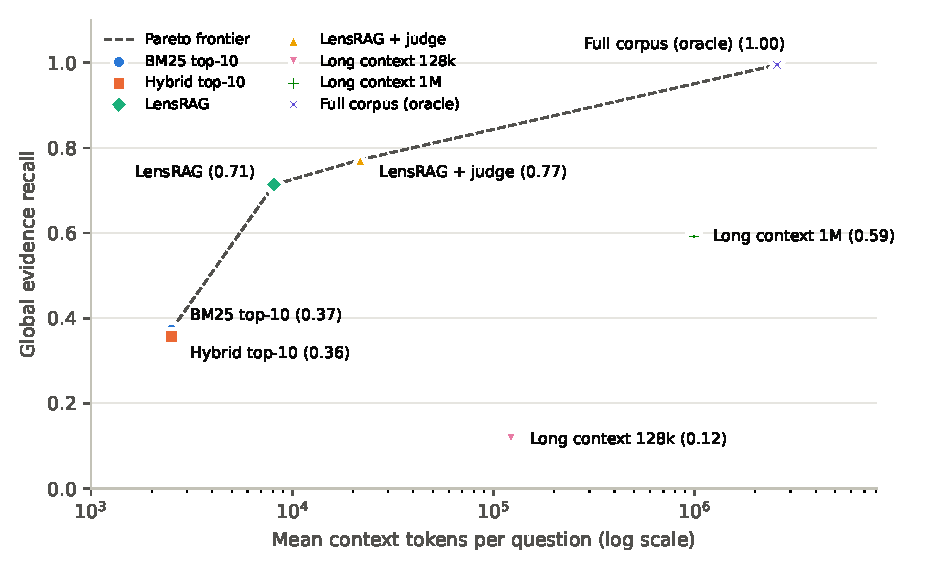
\includegraphics[width=0.9\textwidth]{figures/cost_recall_L.pdf}
\caption{Cost--performance on tier L: global evidence recall against mean
context tokens per question (log scale). The dashed line is the Pareto
frontier.}
\label{fig:cost}
\end{figure}

The answer level reverses the cost picture. Standard RAG makes one LLM call
per question (2.7k tokens, median 21\,s). LensRAG makes 34 calls on average:
\begin{itemize}
  \item 78.8k tokens per question (91.7k for global questions, 23.9k for
  local);
  \item a median of 6.9 minutes per answer;
  \item a 95th percentile of 26 minutes, driven by Mode B estimates, which
  label 150 records three times each;
  \item 15.0 hours for all 89 answers, against 0.6 hours for standard RAG.
\end{itemize}
With local models this cost is time, not money. With an API model it would be
about 30 times the token cost of standard RAG, for no gain in exact match in
this configuration.

\section{Error Analysis}
\label{sec:errors}

LensRAG answered 33 of 88 scored questions exactly. The 55 misses fall into
four groups (Table~\ref{tab:errors}).

\begin{table}[htbp]
\centering\small
\caption{Causes of LensRAG's exact-match misses on tier L. ``Evidence
missed'' uses the retrieval benchmark's LensRAG run as a proxy, which has the
same index and planner.}
\label{tab:errors}
\begin{tabularx}{\textwidth}{@{}lrX@{}}
\toprule
Cause & $n$ & Typical question types and examples \\
\midrule
Evidence missed & 21 & version difference (5), temporal (3), rank (3), theme, conflict; e.g.\ Q048 found 1 of 5 future-dated circulars \\
Evidence found, wrong value & 13 & local (3), count, extremum; e.g.\ Q008 and Q012 averaged several values for a single-country question \\
Mode B estimate off & 13 & count, aggregate, sentiment shift; e.g.\ Q077 estimated 417 tickets where the gold is 42 \\
Partly right (set F1 $>0$) & 8 & theme (4), filter, rank; e.g.\ Q019 returned the four correct countries plus one extra \\
\bottomrule
\end{tabularx}
\end{table}

\begin{itemize}
  \item \emph{Local questions lost.} Four local questions were answered wrongly.
  \begin{itemize}
    \item In two (Q008, Q012), the answer is an average of several values
    (9.33 versus the gold 6). This suggests the single-country lookup was
    treated as an aggregate. The question type chosen by the classifier is
    not recorded in the answer log, so this is inferred, not observed.
    \item In one (Q014), the answer took a stale handbook value (INR\,500)
    instead of the current policy (INR\,600).
  \end{itemize}
  Standard RAG answers the same questions directly from the top chunk.
  \item \emph{Sampled labels are biased.} The gold value fell inside the
  reported 95\% interval for only half of the 18 answers that carry an
  interval, against 95\% for well-calibrated intervals. The intervals
  express sampling error but not labelling error. When the 14B model labels
  records systematically wrongly, the interval is narrow and wrong. Examples
  are Q080 (estimated share 0.76, gold 0.04) and Q089 (1{,}087 versus 819).
  \item \emph{Temporal and version questions.} LensRAG scored 0.20 on
  temporal questions against 0.60 for standard RAG, and in most misses the
  evidence was not retrieved. A likely cause is the scoping step. It
  excludes superseded documents unless the question names a version, but
  temporal questions name a date instead, so the circular or earlier
  version that holds the answer can be filtered out.
  \item \emph{Where LensRAG helped.} It was more accurate on count (0.38
  versus 0.12) and aggregate questions (0.20 versus 0.00), and had higher
  set F1 on theme (0.61 versus 0.39), version-difference (0.54 versus 0.33)
  and rank questions. These are the question types that need many
  documents.
\end{itemize}

\chapter{Discussion}
\label{ch:discussion}

\section{Interpretation}
\label{sec:interpretation}

The results separate two claims that are often merged:
\begin{itemize}
  \item \emph{Coverage.} LensRAG solves the coverage problem it was designed
  for. Entity-scoped retrieval over context-enriched chunks roughly doubles
  the evidence that reaches the generator on large corpora, at a small
  fraction of long-context cost.
  \item \emph{Correctness.} Coverage alone does not produce correct
  aggregate answers. Between retrieval and the answer sit classification,
  extraction, labelling and formatting, each done here by a 3B--32B local
  model. Errors at each step compound: a pipeline of individually reasonable
  steps can equal a single top-$k$ call in accuracy while costing 30 times
  more.
\end{itemize}
The error analysis shows where the losses occur:
\begin{itemize}
  \item routing local questions down the global path;
  \item filtering out superseded documents that temporal questions need;
  \item treating sampling error as the only uncertainty in estimates.
\end{itemize}
Each is a design choice that can be changed, rather than a limit of the
approach.

\section{Implications for Practitioners}
\label{sec:practice}

\begin{itemize}
  \item \textbf{Route conservatively.} Send a question down the aggregation
  path only when it is clearly global, and default to standard RAG
  otherwise. Standard RAG answered every local question correctly.
  \item \textbf{Use coverage retrieval when a corpus outgrows the context
  window.} When the whole corpus fits (tier S here), long-context prompting
  or top-$k$ retrieval with a larger $k$ is simpler and as good.
  \item \textbf{Treat estimates from LLM labels as biased, not only noisy.}
  Validate the labelling model on a small hand-labelled set before reporting
  intervals.
  \item \textbf{Size models to the step.} Small models are adequate for
  extraction with verbatim spans, but classification errors are costly
  because they change the whole path. The classifier is the step where a
  stronger model pays off.
  \item \textbf{Measure answers, not only retrieval.} Evaluating retrieval
  alone would have shown a clear win here.
\end{itemize}

\section{Implications for Research}
\label{sec:research-implications}

Benchmarks for corpus-level question answering should report retrieval
coverage and answer accuracy separately, since they diverge sharply here.
Interval coverage is a useful and rarely reported check of estimate
calibration. The synthetic, ledger-first corpus made exact answers possible
for counting, ranking and sentiment-shift questions over thousands of
records, which hand-annotated corpora cannot provide at this scale.

\section{Limitations}
\label{sec:limitations}

\begin{itemize}
  \item \textbf{Configuration.} The answer-level run used local open-weight
  models up to 32B and omitted the reranker, NER, NLI and sentiment
  components. Results with stronger or API models, or with all components,
  may differ.
  \item \textbf{Runs and sample size.} Answers were generated in a single
  run. The question set is small, with 72 global questions on tier L.
  \item \textbf{Baselines not run.} No GlobalRAG-style baseline and no
  answer-level long-context baseline were run.
  \item \textbf{Corpus.} The corpus is synthetic and template-generated, so
  its phrasing is more regular than real documents.
  \item \textbf{Conflict and faithfulness measures.} Conflict-flag precision
  and recall, and claim-level faithfulness, were not measured against human
  judgements.
\end{itemize}

\section{Ethical, Legal and Societal Considerations}
\label{sec:ethics}

\paragraph{Data.}
The corpus is fictional and contains no personal data. In a real deployment,
HR documents such as grievances, exit interviews and survey comments are
personal data under regulations such as the GDPR and India's Digital
Personal Data Protection Act (DPDP).

\paragraph{Design choices that help.}
\begin{itemize}
  \item Self-hosting keeps documents on the organisation's infrastructure.
  \item Aggregate answers expose counts and shares, not individual records,
  although small groups can still identify people. A minimum group size
  should be enforced.
  \item Estimates are labelled as such and carry intervals.
\end{itemize}

\paragraph{Risks and regulation.}
Automated sentiment and theme analysis of employee feedback could be used for
surveillance or to judge individuals. LensRAG should be used for
organisation-level questions, with human review of any decision. Under the
EU AI Act, AI systems used to monitor or evaluate workers are classed as
high-risk.

\chapter{Conclusion and Future Work}
\label{ch:conclusion}

\section{Summary of Contributions}
\label{sec:summary}

\begin{itemize}
  \item \textbf{Benchmark.} An 89-question HR benchmark over a 2.6M-token
  synthetic corpus in three tiers, with answers computed from a ledger.
  \item \textbf{Method.} LensRAG, a schema-free method that combines
  context-enriched chunks, entity-scoped coverage retrieval, computation in
  code, sampled estimates with intervals, consistency-filtered generation,
  and verification. It has pluggable models per role and runs fully on
  local hardware.
  \item \textbf{Findings.}
  \begin{itemize}
    \item Standard RAG answers local questions far better than global ones
    (1.00 versus 0.28 exact match).
    \item LensRAG doubles global evidence recall on large corpora at 0.3\% of
    long-context cost.
    \item With local models this did not raise exact match. Set F1 improved,
    local accuracy fell, and the failure modes are identified.
  \end{itemize}
  \item \textbf{Software.} An open, tested implementation (108 tests) with a
  one-command experiment.
\end{itemize}

\section{Future Work}
\label{sec:future}

\begin{enumerate}
  \item Re-run the answer level with all components enabled, and with a
  stronger API model for classification and answering, to separate method
  from model capacity.
  \item Route conservatively: fall back to standard RAG unless the question
  is clearly global, and add a check that a local question returns a single
  value.
  \item Keep superseded documents in scope for date questions, and resolve
  them by effective date.
  \item Calibrate Mode B intervals for labelling error by checking the
  labeller on a hand-labelled sample and widening the intervals accordingly.
  \item Measure conflict-flag precision and recall against the twelve
  planted conflicts.
  \item Add a GlobalRAG-style baseline, repeat runs with several seeds, and
  run the planned ablations.
  \item Evaluate on a second domain using the legal configuration.
\end{enumerate}

\section{Publication Plan}
\label{sec:publication}

The target is an arXiv preprint (cs.CL, cross-listed to cs.IR) followed by a
workshop on retrieval or enterprise NLP. The condensed paper will have six
parts:
\begin{enumerate}
  \item problem and benchmark;
  \item method;
  \item retrieval-level results across tiers;
  \item answer-level results and error analysis;
  \item cost;
  \item limitations.
\end{enumerate}
The corpus, gold set and code will be released with it.

%---------------------------------------------------------------------
% BIBLIOGRAPHY
%---------------------------------------------------------------------
\bibliographystyle{plainnat}
\bibliography{references}

%---------------------------------------------------------------------
% APPENDICES
%---------------------------------------------------------------------
\appendix
\chapter{Individual Contribution Statement}
\begin{tabularx}{\textwidth}{@{}lX@{}}
\toprule
\textbf{Member} & \textbf{Contribution (CRediT taxonomy)} \\
\midrule
Member One   & Conceptualisation, methodology, writing --- original draft \\
Member Two   & Software, architecture, deployment \\
Member Three & Data curation, evaluation, visualisation \\
Member Four  & Security testing, governance mapping, validation \\
Member Five  & LLMOps, cost analysis, writing --- review \& editing \\
\bottomrule
\end{tabularx}

\chapter{Weekly Progress Log}
\begin{longtable}{@{}p{1.2cm}p{5.5cm}p{5.5cm}p{3cm}@{}}
\toprule
\textbf{Week} & \textbf{Planned} & \textbf{Achieved} & \textbf{Advisor notes} \\
\midrule
\endfirsthead
\toprule
\textbf{Week} & \textbf{Planned} & \textbf{Achieved} & \textbf{Advisor notes} \\
\midrule
\endhead
1 & Kick-off; Closing Project Title and Project Scope, Start of literature scan & & \\
2 & 25 research articles research complete & & \\
3 & 50 research articles research complete & & \\
4 & Introduction and Literature Survey Complete & & \\
5-6 & Getting Foundations for the Project Correct& & \\
7 & Foundations Complete& & \\
8--10 & Experiments & & \\
11--12 & Analysis & & \\
13--14 & Writing; arXiv submission & & \\
\bottomrule
\end{longtable}

\chapter{Reproducibility Checklist}
\begin{itemize}[label=$\square$]
  \item Code and configuration released under an open licence at \url{\RepoURL}.
  \item Exact model identifiers, versions and access dates recorded.
  \item Random seeds and number of runs reported for every result.
  \item Datasets released or access instructions provided; licences stated.
  \item Cost (tokens, USD, GPU-hours) reported per experiment.
  \item Prompts and judge instructions included verbatim in the appendix.
  \item Human-annotation protocol and agreement statistics reported.
\end{itemize}

\chapter{Prompts, Judge Instructions and Additional Results}
Include all prompts verbatim, extended tables and figures.

\end{document}
